\documentclass[11pt]{article}
\usepackage{graphicx}
\graphicspath{{./graphs/}}
\usepackage{float}
\usepackage[left=3cm,right=3cm]{geometry}
\usepackage[font=scriptsize]{caption}
\usepackage{amsmath}
\usepackage{array}
\usepackage{multirow}
\usepackage{authblk}
\usepackage{lineno}
\usepackage{cite}
\usepackage{longtable}
\usepackage{subcaption}


\title{The Cubic Polynomial Regression Outperforms Gompertz Equation in Model Fitting of Bacterial Populations}

\author{Cherie Yu}

\affil{Imperial College London}

\date{3 December 2021}

\begin{document}
\maketitle

\pagebreak
\begin{abstract}
    Population growth rates are often used as a response variable to observe and predict changes to 
    population density and abundance. Mathematical models are applied in food microbiology to 
    determine the growth of bacterial populations for the basis of food safety. This study aims 
    to compare how well phenomenological and mechanistic theory models fit to population growth data 
    of bacterial species. By sampling starting parameters from a normal distribution, the polynomial 
    cubic, quadratic and Gompertz equation was successfully fitted to 255 of the 284 unique ID datasets. 
    The Akaike Information Criterion (AIC) was calculated for model comparison. Across all the datasets, 
    the phenomenological cubic equation had the highest total of best fitted growth curves, while 
    the Gompertz model ranked second. This study shows that the mechanistic model has underperformed 
    for unevenly distributed bacterial growth data with small sample sizes and species that demonstrated 
    a death phase. We conclude that model fitting is dependent on the quality of the 
    experimental data. We suggest that model fitting in microbiology should also consider 
    phenomenological models in an area that is rather heavily dependent on mechanistic theories. 
\end{abstract}

\section{Introduction}\\ 

\linenumbers
Population growth rates are used to observe trends in population density and abundance, from 
whether these variables are changing, to the rate they occur \cite{sibly_population_2002}. In addition, population 
growth rates are often applied to predict future projections on population sizes \cite{sibly_population_2002}. Population 
growth rates is important to the application of scientific topics ranging from population ecology, 
conservation biology, food microbiology, evolutionary biology and more \cite{sibly_population_2002,sibly_population_2002-1}. For example, 
population growth rate can be used as a response variable to analysis the success of the invasion 
of maladaptive traits into a resident population \cite{sibly_population_2002-1}.Especially in response to current changing 
conditions that may alter population dynamics e.g climate change, we need to be able to identify 
drivers to the process of population growth, thus helping to prioritize and target management actions \cite{eacker_assessing_2017}. 
In microbiology, modelling bacteria populations have formed the basis of food safety. Being able 
to effectively give realistic predictions of microbial growth during food storage over a range of 
environmental conditions have allowed the minimizing of ineffective, expensive and slow laboratory 
challenge testing of foods \cite{soboleva_predictive_2000,baranyi_mathematics_1995,perni_estimating_2005}. 

Measuring bacteria growth is a measure of all cellular processes and captures how the cells adapts and 
survive in their environmental niches \cite{tonner_bayesian_2020}. As exemplified in figure \ref{fig:mesh1}, bacterial growth in batch culture often assumes a sigmoid growth 
function with three growth phases captured by three parameters: lag phase is where no growth occurs in which 
bacteria undergoes physiological and regulatory processes that is needed for optimal growth, exponential
phase is where there is accelerating rapid growth in a certain period of time (lag time, also denoted as $\lambda$),
thus reaching a maximal value ($\mu m$) \cite{rolfe_lag_2012}. The final phase is the stationary phase where the carrying capacity ($A$) is reached, 
growth rates decreases and reaches 0 where nutrients has been exhausted \cite{tonner_detecting_2017,zwietering_modeling_1990}.  

    \begin{figure}[H]
    \centering
    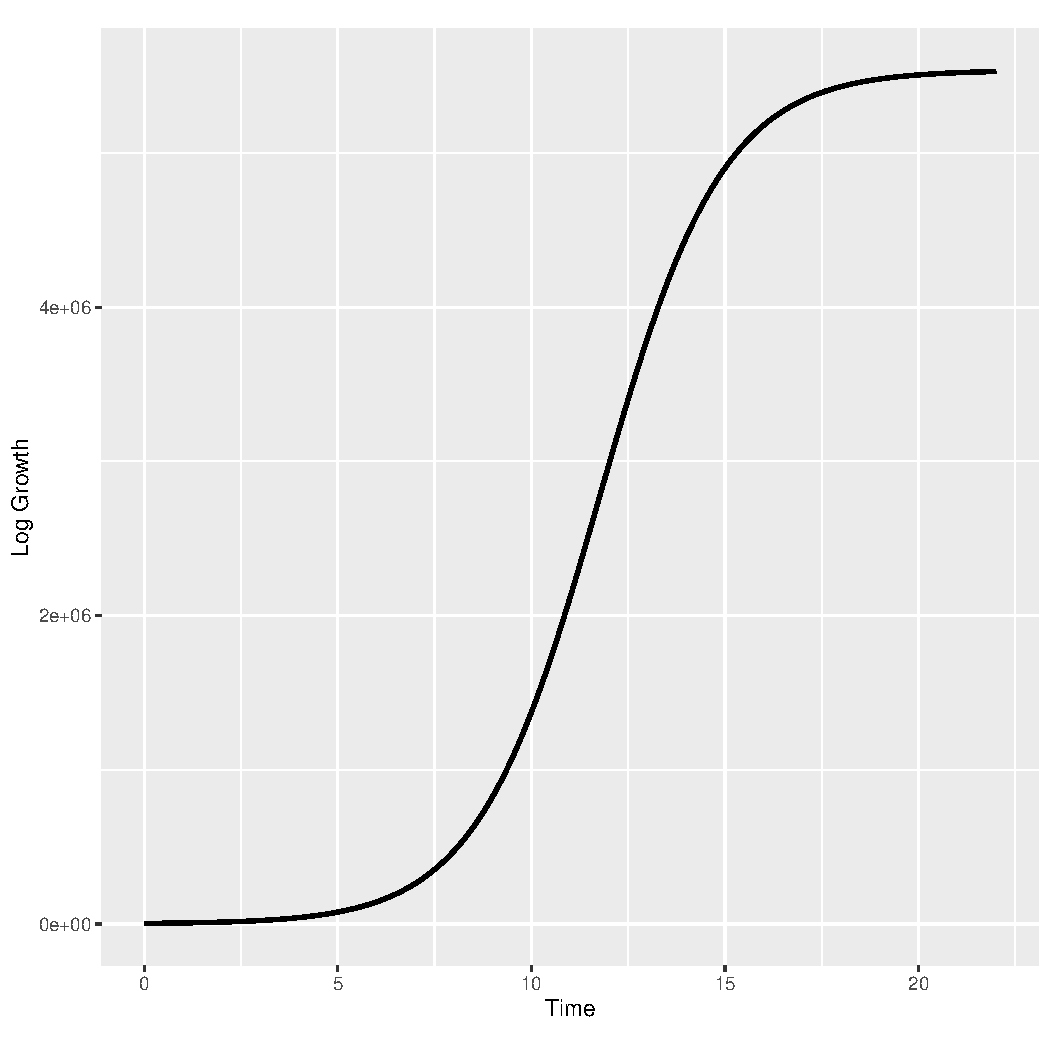
\includegraphics[height=10cm,width=10cm]{example_data_logistic}
    \caption{This figure represents a sigmoid growth curve using example logistic data. The three growth phases are captured here by the three parameters: the lag phase is where no growth occurs and is captured by the lag time ($\lambda$).
    $\mu m$ is the maximum population growth rate which can be captured by fitting a linear regression line through ($\lambda$) and finding the slope. The last phase is the stationary phase ($A$) where growth rate reaches 0.}
    \label{fig:mesh1}
    \end{figure}

Previous work has proposed a variety of mathematical models in the form of algebraic curves to describe 
microbial growth, expressed by functions and equations \cite{soboleva_predictive_2000,peleg_microbial_2011}.In this study, I have split such 
models into two distinct forms: phenomenological models and mechanistic theory models. Phenomenological 
models uses a mathematical function that is fitted to the data to describe the underlying biological process \cite{white_should_2019}.
In contrast, mechanistic models include hypothesis-based parameters that have a biological interpretation 
and explicitly tracks the process of a biological system \cite{geritz_mathematical_2012}. The aim of this study is to compare how well 
these two different types of mathematical models fit to population growth data across bacterial species. A 
large part of the literature has been involved in analysing the power between different mechanistic theories 
in modelling bacterial growth, while phenomenological models are often absent in such context \cite{gibson_predicting_1988,adair_comparison_1989,labuza_growth_1993,mackey_effect_1988}.Although
phenomenological models have substantial predictive power, it can also risk not being validated for any
biological systems due to the generality of their parameters, especially if a prediction is outside the known 
parameters \cite{heitzer_utility_1991,schiraldi_phenomenological_nodate,geritz_mathematical_2012}. In mathematical models, the less number of parameters there are, the greater the explanatory
power. The more meaningful and intuitive the parameters of a model are, the more phases of microbial growth
is covered, providing highly accurate models \cite{esser_modeling_2015}. For such reasons, it can be hypothesized that mechanistic
models can be a better fit within bacterial populations that demonstrate a predictive growth 
curve. The objectives of this study were to (1) fit a quadratic and cubic model to the species datasets (2) 
fit a mechanistic Gompertz model (3) compare the models using the calculated Akaike Information Criteria 
(AIC). 

\section{Materials \& Methods}

\noindent\textbf{Theory} \\

Two phenomenological models were used in this study: cubic and quadratic equation. The cubic equation were
fitted using a third degree polynomial regression model and the quadratic equation uses a second order
polynomial form (parabolic curve). \\

The cubic equation is: \\
    \begin{equation}
    y = at^3 + bt^2 + ct + d 
    \end{equation}

The quadratic equation is: \\
    \begin{equation}
    y = bt^2 + ct + d 
    \end{equation}

\noindent where $y$ = population abundance at $t$, $t$ = time and $a$ $b$ $c$ $d$ are regression coefficients. The number of free 
parameters are 4 and 3 respectively. \\

The Gompertz model is one of the most frequently used non-linear sigmoid model fitted to growth curves \cite{gompertz_xxiv_1825}. 
Originally used to describe human mortality rates, it has now been re-parametrized to be applicable within 
modelling bacteria growth, becoming one of the most common mechanistic models to be used by microbiologists \cite{tjorve_use_2017,gibson_predicting_1988}.
(17)(A) \\

Provided by the literature, the modified Gompertz equation is represented by the general equation: \\
    \begin{equation}    
    log(N_{t}) = N_{0} + (N_{max} - N_{0})e^{-e}^{r_{max}exp(1)\frac{t_{lag}-t}{(N_{max} - N_{0})log(10)}+1}
    \end{equation}
   
\noindent where $N_{t}$ is the population size at time $t$, $N_{0}$ is the initial population size during the lag phase,
$N_{max}$ is the largest population size when the carrying capacity is reached, $r_{max}$ is the rate of exponential growth,
$t_{lag}$ is the $x$ intercept (time) to the tangent of the slope of the exponential growth. \\ 

\noindent\textbf{Data} \\

The dataset contains measurements of change in biomass or number of cells of microbes over time(hours). Data was collected 
through lab experiments across the world, citied from ten research papers \cite{bae_growth_2014,bernhardt_metabolic_2018,roth_wheaton_1962,galarz_predicting_2016,gill_growth_1991,silva_modelling_2018,sivonen_effects_1990,stannard_temperaturegrowth_1985,zwietering_modeling_1994,phillips_relation_1987}.
Single population growth rate curves are identified by unique temperature-species-medium-citation-replicate combination IDs. A total of 284 
unique IDs was isolated, identified as ID 0 to 284. Using Python 3.9, I eliminated any negative time and population 
data and $NaN$ values due to not making any meaningful biological sense.\\

\noindent\textbf{Model Fitting}\\

All model fitting was achieved through utilizing Python 3.9. The modified Gompertz equation (3) was fitted to 284 unique ID 
using the non-linear least squares regression. I used the Levenberg–Marquardt algorithm of minimization, which is the default 
algorithm for Python $lmfit$ function.  The Levenberg-Marquardt algorithm is an effective 
hybrid technique in solving non-linear equations. It uses both Gauss-Newton and steepest descent approaches to converge 
to a minimized, optimal solution \cite{wilson_chapter_2013}. For each unique ID, the four starting values ($N_{0}$, $N_{max}$, $r_{max}$, $t_{lag}$)
were estimated by these methods: $N_{0}$ was calculated by isolating the last value (the starting minimum value) within the sample size of 
the population measure. $N_{max}$ was calculated by finding the maximum value within the population measure. $r_{max}$ and $t_{lag}$
was calculated by sampling values within a normal distribution ($N$ = 100, $\mu$ = $r_{max}$ or $t_{lag}$, $\sigma$ = 0.1), then fitted  
to find the best minimized parameters (refer to table \ref{table:3} in the supplementary data for all minimized parameters from the Gompertz equation). 
Out of 284 ID, I was unable to find a suitable minimized starting values for 10 unique datasets
(ID 4,14,16,20,88,280,281,282,283,284), therefore was omitted from further data processing. This resulted in 274 unique datasets remaining. 
For datasets with a sample size of less than the numbers of free parameter in equation (3) ($df$ = 0), an output of $NaN$ was given due to 
inadequate sample size for data analysis. Similarly, the cubic (1) and quadratic (2) equations was fitted to the remaining dataset 
using the default least squares regression (Levenberg–Marquardt algorithm). All datasets were successfully fitted given the 
estimated starting values of 1. However, unique datasets with the sample size of less than 4 and 3 ($df$ = 0) respectively was given an output of $NaN$.\\ 

\noindent\textbf{Model Selection and Comparison}\\

Model selection was established using a selection criterion: AIC, or rather $AIC_{c}$ \cite{burnham_multimodel_2004}. AIC is a numerical value by which to 
rank competition models in term of information loss. It is used in comparison with other AIC values, where the lowest 
represents the best approximating model \cite{symonds_brief_2011}. In my study, instead of AIC, $AIC_{c}$ was used. When \(\frac{n}{K}<40\) where $n$ = sample size,
$K$ = total number of parameters in the most complex model, $AIC_{c}$ is recommended. $AIC_{c}$ is the small 
sample (second-order bias correction) version of AIC. By using AIC on data with small sample sizes, it increases the change 
of overfitting \cite{burnham_multimodel_2004}.\\

Recent versions of statistical software packages provide AIC values when generating model fitting. AIC values was extracted 
from the cubic, quadratic, Gomepertz model during model fitting. To calculate $AIC_{c}$: \\

    \begin{equation}    
    AIC = -2(ln(likelihood))+2K(\frac{n}{n-K-1})
    \end{equation}\\

    \begin{equation}    
    AIC_{c}= AIC(\frac{n}{n-K-1})
    \end{equation}\\

\noindent where $n$ is the sample size, $K$ is the number of free parameters in the model.\\

AIC scores are often shown as $\triangle$AIC. The individual AIC and $AIC_{c}$ values are not interpretable on its own as they have scaling 
issues and are affected by different sample sizes. Therefore, $AIC_{c}$ was rescaled by this equation: \\

    \begin{equation}    
    \triangle_{i}= AICc_{i} - AICc_{min}
    \end{equation}\\

\noindent where $AICc_{min}$ is the smallest $AIC_{c}$ value between candidate models. $\triangle_{i}$ is the information loss experienced if we were 
using the fitted model $i$. This transformation will result in the best fitted model to have $\triangle_{i}$ = 0. The larger the $\triangle_{i}$, the less 
plausible the fitted model is an accurate candidate model for the given dataset \cite{burnham_multimodel_2004}. In addition, Akaike Weight ($w_{i}$) was calculated as 
the probability that the model chosen is the best model given the data and the set of candidate models \cite{wagenmakers_aic_2004}.\\

The equation is given below:\\

    \begin{equation}    
    w_{i}= \frac{exp(-\triangle_{i}/2)}{\sum_{r=1}^{R}exp(-\triangle_{r}/2)}
    \end{equation}\\

\noindent where $\sum_{r=1}^{R}exp(-\triangle_{r}/2)$ is the sum of the value across all models. \\ 

Using R studios, I then compiled a summary table of all the calculated AIC values for each of the unique 274 datasets. 
However during the process of $AIC_{c}$ calculations, I eliminated two datasets (ID 200,212) for having a sample size 
less than the number of free parameters in the quadratic equation ($N<$3), which is too small for any meaningful analysis. 
In addition for 10 data sets, $-Inf$ and $Inf$ was outputted. From a closer look, it was due to $n$ being divided by a total value 
of 0 or less. Along with any datasets with only one successfully calculated AIC model ($N<$4), a total of 18 unique data 
sets was eliminated from my final table which demonstrates the best fitted model for each ID. \\

\noindent\textbf{Computing Languages and Tools}\\

Data Wrangling, model fitting, graphing and AIC calculations was performed in Python 3.9. AIC tables was created in R 4.1.2 
using R Studio. Sample graph (figure x) was created in R 4.1.2. Specific packages used within each computing languages can 
be found in README.md.

\section{Results}

\noindent\emph{(1,2)Fitting phenomenological and mechanistic mathematical models}\\

Out of the 284 unique IDs from the original dataset, I managed to successfully fit 255 IDs with both phenomenological and mechanistic
models. All datasets that were successfully fitted had a sample size of N>=5. All curves were plotted with the residuals and 
overlaid with the original dataset points. Some examples of model fitting is shown in Figure \ref{fig:fig2}.\\

\begin{figure}[ht]
    \begin{subfigure}[b]{0.5\linewidth}
        \centering
        \includegraphics[width=0.75\linewidth]{graph0}
        \caption{ID 0 with species \emph{Chryseobacterium balustinum} \cite{bae_growth_2014}}
        \label{fig2:a}
        \vspace{4ex}
    \end{subfigure}%%
    \begin{subfigure}[b]{0.5\linewidth}
        \centering
        \includegraphics[width=0.75\linewidth]{graph1}
        \caption{ID 1 with species \emph{Enterobacter.sp.} \cite{bae_growth_2014}}
        \label{fig2:b}
        \vspace{4ex}
    \end{subfigure}
    \begin{subfigure}[b]{0.5\linewidth}
        \centering
        \includegraphics[width=0.75\linewidth]{graph2}
        \caption{ID 2 with species \emph{Pantoea agglomerans.1} \cite{bae_growth_2014}}
        \label{fig2:c}
        \vspace{4ex}
    \end{subfigure}%%
    \begin{subfigure}[b]{0.5\linewidth}
        \centering
        \includegraphics[width=0.75\linewidth]{graph3}
        \caption{ID 3 with species \emph{Pantoea agglomerans.2} \cite{bae_growth_2014}}
        \label{fig2:d}
        \vspace{4ex}  
    \end{subfigure}
    \caption{Figures of model fitting using phenomenological and mechanistic models for ID 0 to 3. Each line represents a specific mathematical model: yellow represents the quadratic equation,
    green is the cubic equation, blue is the mechanistic Gompertz equation. Datapoints are represented by the black crosses. Points are layed on each theoretical model to compare as residuals with the datapoints.}
    \label{fig:fig2}
\end{figure}

\noindent\emph{(3)Model comparison using Akaike Information Criteria}\\
    \begin{table}[htb]
        \caption{The total number of each best fitted models across all 255 unique datasets ranked in order from highest to lowest. The cubic mathemataical equation was
        choosen as the best fitted model for the highest number of IDs. This ranking was based on comparisons of $AIC_{c}$ scores}
        \centering 
        \begin{tabular}{ | m{3cm} | m{12em} | }
            \hline
            Model & Total Number of Each Best Fitted Model Across All ID Based on $AIC_{c}$ Scores \\
            \hline
            Cubic & 168 \\ 
            \hline
            Gompertz & 82 \\
            \hline
            Quadratic & 5 \\
            \hline
            Total & 255 \\
            \hline
        \end{tabular}
    \label{table:1}
    \end{table} \\ 

Table \ref{table:4} in supplmentry data demonstrates the best fitted model from each ID identified by the lowest $AIC_{c}$ score. Table \ref{table:1} further ranks
the three mathematical models by how many times a given model fits best across all unique datasets. From my study, the phenomenological cubic 
model fits best for the highest amount of ID bacterial datasets. 65\% of the ID are best fitted with a Cubic model, 32\% fitted with the 
Gompertz model, while only 3\% of the ID is best described with the quadratic model (ID 58,70,214,217,239). \\

    \begin{table}[htb]
        \caption{Total number of pairs between best fitted model and model with $AIC_{c}<$2 across all ID}
        \centering 
        \begin{tabular}{ | m{6em} | m{8em} | m{8em} |  }
            \hline
            Best Fitted Model & Models with $AIC_{c}$ values with $<$2 & Total Number of IDs \\
            \hline
            Cubic & Quadratic & 1 \\ 
            \hline
            Cubic & Gompertz & 3 \\
            \hline
            Quadratic & Cubic & 4 \\
            \hline
            Gompertz & Cubic & 7 \\
            \hline
            \multicolumn{2}{|c|}{Total} & 15 \\
            \hline
        \end{tabular}
    \label{table:2}
    \end{table} \\ 

Comparing the $\triangle$AICc of candidate models between each dataset ID, it was observed that some of the differences between the scores were $<$2. 
Full list of all mathematical models in all unique IDs with their $AIC_{c}$ values can be found in supplementary table \ref{table:5}.  Highlighted
by Burnham and Anderson 2002, when a variable with poor explanatory power is added to a model, an output of $\triangle$AICc$<$2 can 
occur \cite{burnham_basic_2002,arnold_uninformative_2010}. Only when the differences are $>$2 is considered significant \cite{wyss_seismicity_2012}. 
In table \ref{table:2}, I can see that 15 IDs demonstrated ∆AICc values that are not significantly different. Within those 15
unique IDs, 7 of those indicated that Gompertz model was the best model fitted with the given data, however they were insignificantly different in comparison
to the cubic model. 4 out of the 5 best fitted quadratic model was not significantly different from the cubic model. While the best fitted cubic mode of 3 and
1 IDs was not significantly different from the Gompertz and quadratic model, respectively.

\section{Discussion}\\

Microbial growth is an area extensively studied in food microbiology due to causing the most common food poising \cite{buchanan_when_1997,xiong_comparison_1999}. The use of mathematical models
in fitting and predicting experimental data can help describe the behaviour of microorganisms under different environmental conditions (e.g temperature, PH) \cite{zwietering_modeling_1990}.
In my study, I compared how well two different types of mathematical models: phenomenological and mechanistic theory fit across bacterial population
growth data. This was investigated by fitting the quadratic, cubic and Gomepertz equations to each unique ID datasets and calculating the $AIC_{c}$ values. 
The lower the $AIC_{c}$ value, the best model it is out of the candidate set. In contrast to my initial hypothesis, the phenomenological cubic model 
had the highest percentage of being chosen as the best approximate model. The Gompertz equation was ranked second.  

From visual inspection, more than 100 curves were fitted poorly with the Gompertz equation as a horizontal line was produced. For example, figure \ref{fig:fig3} demonstrates 
four IDs (46,68,82,100) with a poor mechanistic curve. This could be mainly due to the quality of data provided for model fitting. Although highly used within the literature, the fit of the Gompertz function can be
greatly affected by quality of the data observations \cite{labuza_growth_1993}. For a good fit of the function, Labuza T.B, Fu B. and Salazar et al. suggested that preferably 15 uniformly spread
data points are required through all growth phases \cite{labuza_growth_1993,salazar_primary_2021}. Murphy et al. tested out this hypothesis by undergoing random deletion of observations
for each growth curve and refitting the Gompertz equation after. They found that fitting curves to \emph{Clostridium botulinum} species required evenly spread data
during the lag, growth and stationary phases. If no counts were made during the growth phase, a sigmoid curve could not be fitted, and this was
observed in data with approximately 10 or less. In addition, if there was no observation in the lag or stationary phases, an unrealistic 
estimate would be produced \cite{murphy_development_1996}. All of my unique IDs had a small sample size, from $N$ = 4 being the smallest, to $N$ = 66 the largest. Even for IDs
(91,90,92,89) with the largest sample size ($N$=66,63,57,54), the Gompertz model did not fit properly. I suggest that this is due to the lack
of observations collected during the lag phase, which unlike ID 90 had, successfully deemed the Gompertz as the best fitted model ($AIC_{c}$ = -216.31). 

\begin{figure}[ht]
    \begin{subfigure}[b]{0.5\linewidth}
        \centering
        \includegraphics[width=0.75\linewidth]{graph46}
        \caption{ID 45}
        \label{fig3:a}
        \vspace{4ex}
    \end{subfigure}%%
    \begin{subfigure}[b]{0.5\linewidth}
        \centering
        \includegraphics[width=0.75\linewidth]{graph68}
        \caption{ID 68}
        \label{fig3:b}
        \vspace{4ex}
    \end{subfigure}
    \begin{subfigure}[b]{0.5\linewidth}
        \centering
        \includegraphics[width=0.75\linewidth]{graph82}
        \caption{ID 82}
        \label{fig3:c}
        \vspace{4ex}
    \end{subfigure}%%
    \begin{subfigure}[b]{0.5\linewidth}
        \centering
        \includegraphics[width=0.75\linewidth]{graph100}
        \caption{ID 100}
        \label{fig3:d}
        \vspace{4ex}  
    \end{subfigure}
    \caption{Examples of IDs with poor model fitting using minimzed parameters, focusing on the Gompertz equation shown by the blue curve. (a,b,c) All shows a negative trail of decline as $t$ increases. 
    (d) ID 100 shows a positive curve however due to the lack of sample size ($N$=6), the mechanistic model struggles to fit.}
    \label{fig:fig3}
\end{figure}

More than 20 of the graphs produced during visual inspection demonstrated a pattern of decline (refer to ($a$),($b$),($c$) in figure \ref{fig:fig3}). This is predicted to be the death phase of 
bacterial species. My modified gompertz equation did not consider incorporating the death phase in explaining bacterial growth curves. As such, 
the model did not fitted the growth well. Additionally, the Gompertz model would not always be compatible
with microbial growth as the model does not extend beyond the stationary phase \cite{gibson_predicting_1988,xiong_comparison_1999}. As such, other models are found to be preferred and more
robust when modelling microbial death kinetics \cite{xiong_comparison_1999}. In the context of batch fermentation where bacterial population demonstrates a death phase,
Salazar et al. found that the phenomenological cubic model best predict the overall dynamics of the experimental data in comparison to other mechanistic
models (Gompertz, Barayani and Vázquez-Murado) based on the results for the $RSS$ (residual sums of squares) $R^{2}$ and AIC value \cite{salazar_primary_2021}.

It can be suggested that the Gompertz model was ranked second in my study due to the quality and type of data provided. As such, the phenological
mathematical models seemed to be a better fit for predicting bacterial species data. However, what if we consider the power of fit between
phenomenological models? From table \ref{table:2}, I can conclude that the result where IDs identifying the quadratic model as the best fit is insignificant.
Instead, both types of phenomenological model (cubic vs quadratic) was similar in their respective datasets ($AIC_{c}<$2). In polynomial equations, previous work has shown mixed 
results regarding model fitting. Murphy et al. found that the cubic model was superior to lower order models (quadratic) in fitting bacterial population 
growth \cite{murphy_development_1996}. While others have shown that quadratic models yield more accurate estimates of growth rate and lag time in noisy data sets \cite{ng_mathematical_1997,gauch_prediction_1993,mcclure_predictive_1997}.
In some cases, the power of the equations to reflect the data was approximately the same \cite{gibson_predicting_1988}. This study is unable to demonstrate a 
detailed comparison between both types of phenomenological model due to limited statistical analysis in the $RSS$ and $R^{2}$ value. 
Nonetheless, this could be investigated in future works as the main goal of model fitting is to choose the best parsimonious model that in its 
simplest state, still correctly predicts experimental results \cite{gauch_prediction_1993,gibson_predicting_1988}. In my study, I did not take into consideration other statistical analysis
such as an $ANOVA$ of the AIC, $RSS$, $R^{2}$ to compare model fits. Consequently, the models predicted in my study might not be the best fit even 
though my starting values were successfully minimized. Future work is recommended in repeating this method with larger and evenly spread 
samples across all bacterial growth stages while including additional in-depth statistical test to achieve more robust conclusions.

The application of mathematical models to population growth data is a widely effective method to investigate how populations respond to 
biological interactions. My investigation highlights the importance of phenomenological equations in food microbiology that often focuses rather
on mechanistic theory models. This provides as a reminder for future studies to consider both types of models in the study of bacterial growth data.
When undergoing the process of model fitting, one should first consider the quality of the experimental data and the type of species under
investigation. Furthermore, a true validation of the model should come from the ability to correctly predict experimental results and can be 
confirmed through independent testing of its parameters \cite{peleg_microbial_2011}.


\bibliographystyle{apalike}
\nolinenumbers
\bibliography{miniproject}
\pagebreak
\section{Supplementary Data}

    \begin{center}
    \begin{longtable}{llllll}
        \caption{Minimized parameters of the Gompertz equation after sampling a normal distribution for all ID and their AIC values}
        \label{table:3}\\
        ID  & $N_{0}$       & $N_{max}$                 & $r_{max}$            & $t_{lag}$      & AIC      \\
        0   & -9349.442  & -1.309                 & 66.501            & -1042.001          & -154.622 \\
        1   & -11.859    & -0.565                 & 0.278             & -65.634            & -210.677 \\
        2   & -4.692     & -0.747                 & 0.15              & 29.309             & -157.373 \\
        3   & -0.824     & -5.562                 & 0.09              & 129.568            & -82.049  \\
        5   & -4191.507  & -0.871                 & 22.573            & -1287.587          & -168.645 \\
        6   & -1.412     & -18.571                & 0.092             & 97.142             & -126.798 \\
        7   & -832.789   & -1.788                 & 6.179             & -704.082           & -123.491 \\
        8   & -2.11      & -107373317.354         & 38936.046         & -4385.96           & -147.611 \\
        9   & -4.211     & -2.225                 & 0.017             & -18.835            & -108.963 \\
        10  & -5.466     & -1.55                  & 0.059             & -13.155            & -151.785 \\
        11  & -1.326     & -100901.294            & 64.952            & -1745.064          & -149.149 \\
        12  & -0.972     & -6.591                 & 0.038             & 140.605            & -177.885 \\
        13  & -4.899     & -4.364                 & 0.279             & 597.086            & -48.289  \\
        15  & -4.69      & -0.886                 & 0.098             & 52.15              & -156.926 \\
        17  & -3.064     & -6.827                 & 0.009             & 223.544            & -142.943 \\
        18  & -6.243     & -1.809                 & 0.032             & -60.178            & -115.305 \\
        19  & -4.946     & -4.408                 & 0.211             & 595.456            & -48.258  \\
        21  & -3514.935  & -1.009                 & 14.423            & -1664.8            & -156.061 \\
        22  & -4.094     & -1.143                 & 0.074             & -21.236            & -111.125 \\
        23  & -3.359     & -0.191                 & 0.822             & 1.39               & -132.213 \\
        24  & -493.282   & 6344.123               & 0.006             & -29656.636         & 0.778    \\
        25  & -1.384     & -1.621                 & -0.003            & 243.116            & 3.566    \\
        26  & -896.956   & 8191.764               & 0.01              & -117276.188        & -5.703   \\
        27  & -1.093     & -1.093                 & -0.051            & 318.351            & 2.586    \\
        28  & -2.057     & -2.057                 & -0.043            & 323.263            & 11.16    \\
        29  & -7168.995  & -1.363                 & 308.138           & -170.33            & -101.357 \\
        30  & -1.651     & -1.845                 & -0.004            & 381.252            & -47.617  \\
        31  & -2.344     & -2.254                 & 1.275             & 292.702            & 5.075    \\
        32  & -664.496   & 7617.267               & 0.008             & -60582.168         & -4.021   \\
        33  & -1.584     & -2.165922005997174e+16 & 51578958951009.05 & -919.843           & -37.117  \\
        34  & -0.719     & -1.003                 & -0.014            & 550.158            & -5.85    \\
        35  & -813.25    & 9997.267               & 0.01              & -43376.924         & -0.231   \\
        36  & -1.052     & -1.052                 & -0.02             & 322.967            & 15.423   \\
        37  & -1.524     & -1.524                 & -0.027            & 322.408            & 25.529   \\
        38  & -0.665     & -37415.751             & 252.687           & -149.901           & -49.753  \\
        39  & -37.179    & 492.541                & 0.001             & 103.472            & -32.987  \\
        40  & -3.52      & -1.511                 & 0.025             & -20.775            & -18.703  \\
        41  & -3.022     & -0.286                 & 0.17              & -8.734             & -49.592  \\
        42  & -3207.061  & -1.572                 & 46.88             & -437.045           & -62.618  \\
        43  & -1.042     & -16.043                & 0.155             & 38.685             & -40.852  \\
        44  & -2.263     & 30695.275              & 79.679            & 735201.506         & 10.875   \\
        45  & -0.87      & -1.334                 & -0.082            & 299.739            & 12.284   \\
        46  & -1.729     & 16.729                 & -0.053            & -980.083           & 15.051   \\
        47  & 25680.304  & -1.901                 & -2100.69          & -2796041.394       & 18.565   \\
        48  & -2.691     & -15863366.403          & -141216.352       & 24533231.854       & 15.608   \\
        49  & 33.314     & -1.752                 & -1.682            & -3701.744          & 13.241   \\
        50  & -4.649     & -1.692                 & 0.346             & -2.921             & -28.264  \\
        51  & -3122.277  & -1.221                 & 257.455           & -80.567            & -54.053  \\
        52  & -2.448     & -1.255                 & 0.079             & 334.928            & -3.165   \\
        53  & -2.526     & 570198.252             & 375.753           & 30166863.242       & 4.245    \\
        54  & -2.331     & -1.255                 & 0.088             & 334.989            & -1.136   \\
        55  & 5529.539   & -2.172                 & -332.132          & -748200.732        & 13.212   \\
        56  & -83901.248 & -0.692                 & -3519.521         & 183735.801         & 4.71     \\
        57  & -3.306     & -0.434                 & 0.203             & -5.537             & -4.166   \\
        58  & -1.915     & -4.318                 & -0.363            & -166.841           & 37.979   \\
        59  & -4.236     & -0.673                 & 1.132             & 3.0                & -47.131  \\
        60  & -1.462     & -1.255                 & 0.039             & 334.727            & 13.112   \\
        61  & -2.773     & 2.183                  & -0.003            & -3745.555          & -4.329   \\
        62  & -2.755     & -1.255                 & 0.06              & 334.851            & 12.334   \\
        63  & -0.826     & -0.826                 & 0.158             & 334.973            & 4.674    \\
        64  & 304.903    & -3.203                 & -14.693           & -44982.258         & 21.841   \\
        65  & -4.552     & -0.845                 & 0.387             & -4.276             & -25.793  \\
        66  & -2.36      & -1.255                 & 0.035             & 334.908            & 10.566   \\
        67  & -1.397     & -0.706                 & -0.034            & 709.134            & 6.445    \\
        68  & -1.93      & -1.255                 & 0.107             & 334.854            & 19.964   \\
        69  & 927812.261 & -1.664                 & -73833.071        & -111779997.404     & 11.936   \\
        70  & -3.235     & -1.255                 & 0.207             & 335.003            & 36.198   \\
        71  & 204.958    & -1.595                 & -10.526           & -23635.416         & 15.579   \\
        72  & -2.781     & 15809.633              & -118.795          & -893381.4          & 9.56     \\
        73  & -2.121     & -1.255                 & 0.074             & 335.039            & -2.303   \\
        74  & 4.452      & -1.951                 & -0.451            & -418.512           & 7.594    \\
        75  & -2.222     & -1.255                 & 0.05              & 334.885            & 6.395    \\
        76  & -2.327     & -1.255                 & 0.074             & 334.846            & -0.085   \\
        77  & -2.507     & -1.255                 & 0.056             & 334.816            & -4.504   \\
        78  & 25.093     & -0.668                 & -1.397            & -3260.889          & 13.123   \\
        79  & -1.298     & -1.255                 & 0.205             & 334.917            & 17.644   \\
        80  & -2.184     & 27140.916              & -186.133          & -1316213.465       & 4.081    \\
        81  & 88.396     & -1.823                 & -4.75             & -10087.375         & 19.715   \\
        82  & -1.212     & -1.212                 & 0.067             & 334.799            & 7.751    \\
        83  & -2.701     & 16.799                 & -0.049            & -1064.414          & -3.934   \\
        84  & -2.977     & -1.255                 & 0.05              & 334.725            & 7.465    \\
        85  & -4.753     & -1.255                 & -0.353            & 334.805            & 12.29    \\
        86  & -2.375     & -1.255                 & 0.136             & 334.976            & 14.45    \\
        87  & -1.627     & 1271043.31             & 6031.48           & 15061524.955       & 11.718   \\
        89  & 8.931      & 46.449                 & -0.073            & -5288.072          & 33.906   \\
        90  & 9.752      & 7.04                   & 0.085             & 197.715            & -199.145 \\
        91  & 8.861      & 8.861                  & -0.111            & 179.366            & -46.193  \\
        92  & 7.483      & 8.284                  & -0.464            & -109.975           & 20.84    \\
        93  & -0.123     & 8.159                  & 0.046             & 148.328            & -30.14   \\
        94  & 5.511      & -0.506                 & 0.055             & 386.433            & -12.501  \\
        95  & 4.127      & 2334.808               & 4.981             & 58706.367          & 37.746   \\
        96  & 4.11       & -5.158                 & -0.232            & 974.055            & 29.853   \\
        97  & 710.579    & 4.289                  & -31.357           & -90750.36          & 21.433   \\
        98  & 3.824      & 4.127                  & -0.167            & 984.498            & 21.363   \\
        99  & -0.425     & 7.956                  & 0.038             & 87.536             & -31.315  \\
        100 & 4.36       & 291.447                & -0.108            & -15527.349         & 14.707   \\
        101 & 7.193      & -1.939                 & 0.093             & 245.504            & -24.775  \\
        102 & 4.321      & 1.34                   & -0.115            & 334.871            & 31.266   \\
        103 & 907.623    & 4.221                  & -41.512           & -113274.339        & 30.054   \\
        104 & 4.119      & -0.407                 & -0.223            & 1524.973           & 24.117   \\
        105 & 0.089      & 3.06                   & 0.066             & 191.984            & -33.178  \\
        106 & 3.998      & 4.209                  & -8.565            & 777.481            & 16.76    \\
        107 & 0.018      & 6.423                  & 0.082             & 131.216            & -45.267  \\
        108 & 6.231      & -15.141                & 0.149             & 124.696            & -25.73   \\
        109 & 20.686     & 4.035                  & -1.823            & -2055.041          & 28.709   \\
        110 & 4.121      & 0.622                  & -0.231            & 214.429            & 24.638   \\
        111 & -0.018     & 6.08                   & 0.085             & 114.015            & -27.293  \\
        112 & 6.984      & -2.486                 & 0.076             & 293.903            & -8.4     \\
        113 & 0.195      & 6.464                  & 0.113             & 93.282             & -23.447  \\
        114 & 4.048      & 3.036                  & -3.861            & 304.706            & 35.242   \\
        115 & 4.845      & 0.35                   & -0.403            & 220.64             & 33.293   \\
        116 & 5.003      & 0.733                  & -0.189            & 213.99             & 26.12    \\
        117 & 0.166      & 5.748                  & 0.086             & 138.839            & -42.861  \\
        118 & 4.904      & 3.419                  & -10.701           & -1646.898          & 17.485   \\
        119 & 5.369      & -0.636                 & 0.093             & 229.569            & -45.797  \\
        120 & 3.396      & 22.967                 & -0.01             & -6504.836          & 30.19    \\
        121 & 3.828      & -0.541                 & 230692309.709     & -1191486071114.843 & 27.323   \\
        122 & 6.842      & -3.821                 & 0.383             & 51.751             & -36.516  \\
        123 & 0.211      & 8.047                  & 0.062             & 150.061            & -20.749  \\
        124 & 5.892      & -7605.59               & -484.761          & 33758.417          & 12.408   \\
        125 & 2.944      & 2.944                  & 0.067             & -183.749           & 33.755   \\
        126 & 2.096      & 5.161                  & -0.324            & 408.726            & 28.719   \\
        127 & 5.094      & 284079.416             & 1939.155          & 5048699.068        & 33.525   \\
        128 & 4.141      & -18.404                & -0.31             & 216.565            & 26.915   \\
        129 & 6.336      & -1.102                 & 0.056             & 390.35             & -31.513  \\
        130 & -5358.892  & 57084.113              & 0.061             & -88152.835         & 5.168    \\
        131 & 4.115      & 4.013                  & -0.28             & -115.883           & 34.029   \\
        132 & 2.576      & 3.163                  & -0.972            & 231.761            & 27.736   \\
        133 & 3.291      & -3.369                 & -0.043            & 568.971            & 26.984   \\
        134 & 3.386      & -0.322                 & -2.243            & 214.491            & 19.966   \\
        135 & 5.696      & -1.008                 & 0.054             & 358.22             & -25.003  \\
        136 & 1.006      & 6.319                  & 0.073             & 164.875            & -19.134  \\
        137 & 6.734      & -0.538                 & 0.079             & 262.336            & -33.795  \\
        138 & 3.648      & 22.795                 & -3.814            & -791.069           & 26.695   \\
        139 & -0.255     & 2.896                  & -2.236            & 225.866            & 20.703   \\
        140 & -0.668     & 6.36                   & 0.503             & 14.8               & -12.625  \\
        141 & -0.006     & 7.728                  & 0.075             & 198.094            & -25.463  \\
        142 & 0.232      & 8.214                  & 0.083             & 183.197            & -18.649  \\
        143 & 3.865      & 6.837                  & -0.296            & -43.47             & 36.129   \\
        144 & -1.384     & 3.985                  & -32.515           & 221.826            & 29.985   \\
        145 & 3.561      & 26.645                 & -0.144            & -1759.934          & 24.254   \\
        146 & -1.103     & 2.989                  & -0.619            & 1388.814           & 21.791   \\
        147 & 0.164      & 6.226                  & 0.059             & 162.472            & -32.596  \\
        148 & 7.281      & -0.324                 & 0.128             & 212.831            & -21.451  \\
        149 & 0.268      & 6.191                  & 0.081             & 155.126            & -20.362  \\
        150 & 48.937     & 3.649                  & -0.675            & -1541.825          & 26.244   \\
        151 & 3.8        & -2.79                  & -0.037            & 857.303            & 24.529   \\
        152 & 3.563      & 24.161                 & -0.058            & -3928.374          & 19.085   \\
        153 & 2.675      & 3.955                  & -0.062            & -43.621            & 23.858   \\
        154 & 0.626      & 7.072                  & 0.079             & 151.551            & -18.254  \\
        155 & 0.241      & 8.283                  & 0.104             & 92.258             & -44.676  \\
        156 & 3.533      & 3.533                  & -0.962            & 188.171            & 27.397   \\
        157 & 18493.588  & 3.075                  & -460.426          & -1387035.453       & 20.112   \\
        158 & 0.278      & 6.523                  & 0.623             & 17.749             & -21.076  \\
        159 & 3.195      & 4.025                  & -0.122            & -109.077           & 23.493   \\
        160 & 0.113      & 9.395                  & 0.099             & 163.323            & -0.126   \\
        161 & 4.969      & 17.178                 & -0.088            & -315.742           & 35.166   \\
        162 & -0.126     & 7.938                  & 0.253             & 42.545             & -16.621  \\
        163 & 0.429      & 8.563                  & 0.366             & 23.671             & -26.366  \\
        164 & 3.413      & -0.731                 & -37.85            & 221.568            & 27.502   \\
        165 & 7.329      & -0.538                 & -0.41             & 903.785            & 17.597   \\
        166 & 3.335      & 7.026                  & 1.646             & 1.415              & -20.641  \\
        167 & 4.687      & 3.767                  & 1.023             & 6.198              & -16.294  \\
        168 & 7.767      & -72.591                & -0.135            & 2985.95            & 13.727   \\
        169 & 6.266      & -13.831                & -0.983            & 213.489            & 13.154   \\
        170 & -2.659     & 4.678                  & -0.724            & 214.482            & 5.063    \\
        171 & 7.523      & -1.016                 & -6.294            & 214.404            & 17.099   \\
        172 & 5.627      & -0.541                 & -0.279            & 518.213            & 9.091    \\
        173 & 9.799      & 3.892                  & 3.377             & 4.546              & -20.548  \\
        174 & 10.692     & 1.53                   & 2.705             & 6.381              & -17.045  \\
        175 & 5.917      & -0.514                 & -0.39             & 1067.614           & 8.419    \\
        176 & 9.378      & 4.066                  & 3.287             & 5.6                & -18.068  \\
        177 & 4.502      & -12.769                & -0.535            & 213.617            & 6.113    \\
        178 & 4.815      & 2.0                    & -0.059            & 214.177            & 4.291    \\
        179 & 6.94       & -0.539                 & -0.264            & 616.384            & 12.126   \\
        180 & 6.879      & -10.887                & -23.628           & 214.358            & 15.204   \\
        181 & 8.62       & 3.752                  & 6.202             & 2.399              & -41.651  \\
        182 & 6.45       & -0.541                 & -0.34             & 633.115            & 14.076   \\
        183 & 5.942      & 1.299                  & -0.079            & 214.043            & 15.559   \\
        184 & 5.773      & 46.176                 & -0.145            & -5944.509          & 13.256   \\
        185 & 11.272     & -6518774.952           & 311774.183        & -28.564            & -9.701   \\
        186 & -2.666     & 8.467                  & -0.953            & 214.325            & 12.307   \\
        187 & 7.71       & -14.778                & -1.47             & 213.605            & 13.277   \\
        188 & 6.661      & 6383715.637            & -38390.503        & -499854175.969     & 9.724    \\
        189 & 7.498      & -0.541                 & -33690173.017     & 408526626373.911   & 14.535   \\
        190 & 6.763      & -0.012                 & -0.135            & 692.24             & 13.9     \\
        191 & 9.307      & 1.906                  & 11.006            & 0.966              & -9.48    \\
        192 & 7.638      & -5.084                 & -0.18             & 213.55             & 16.618   \\
        193 & 8.942      & 0.685                  & 12.728            & 0.93               & -8.661   \\
        194 & 6.558      & -11.366                & -3.43             & 213.843            & 13.025   \\
        195 & 7.41       & 412.648                & -1.962            & -45643.507         & 18.208   \\
        196 & 7.274      & 0.66                   & -0.183            & 1011.485           & 15.796   \\
        197 & 2.99       & 2.488                  & 1259.339          & 2512106.027        & 16.32    \\
        198 & 3.783      & 3.239                  & -54.831           & -177012.127        & 19.874   \\
        199 & NaN        & NaN                    & NaN               & NaN                & NaN      \\
        200 & NaN        & NaN                    & NaN               & NaN                & NaN      \\
        201 & NaN        & NaN                    & NaN               & NaN                & NaN      \\
        202 & NaN        & NaN                    & NaN               & NaN                & NaN      \\
        203 & 18.264     & 4.307                  & -0.106            & 214.487            & 15.354   \\
        204 & 3.6        & 0.01                   & 0.177             & 214.353            & 20.167   \\
        205 & -20.423    & 3.25                   & -29.523           & 13378.983          & 19.066   \\
        206 & NaN        & NaN                    & NaN               & NaN                & NaN      \\
        207 & NaN        & NaN                    & NaN               & NaN                & NaN      \\
        208 & 5.382      & -0.655                 & 0.346             & 71.113             & 15.338   \\
        209 & 4.247      & 4.247                  & -0.07             & 71.133             & 12.573   \\
        210 & -89.595    & 3.985                  & 8293.57           & -5468531.163       & 20.362   \\
        211 & NaN        & NaN                    & NaN               & NaN                & NaN      \\
        212 & NaN        & NaN                    & NaN               & NaN                & NaN      \\
        213 & 3.426      & 7.703                  & 0.018             & 1902.728           & 17.824   \\
        214 & 0.033      & 8.06                   & 0.025             & 280.436            & -11.625  \\
        215 & 4.403      & 4.317                  & -0.979            & -594.868           & 32.162   \\
        216 & 0.831      & 6.193                  & 0.096             & 24.494             & -33.605  \\
        217 & 4.398      & 219.96                 & 1.92              & 573.966            & 15.361   \\
        218 & 5.399      & 0.992                  & 0.584             & 54.69              & -32.969  \\
        219 & 0.998      & 9.996                  & -0.034            & -1338.901          & -170.082 \\
        220 & 0.992      & 4.986                  & 0.048             & 126.163            & -70.437  \\
        221 & 0.1        & 5.251                  & 0.086             & -21.175            & -56.405  \\
        222 & 5.839      & 6.06                   & -0.077            & -671.074           & 25.138   \\
        223 & 1.001      & 6.681                  & 0.431             & 45.43              & -31.914  \\
        224 & 1.014      & 1.014                  & -4.583            & 532.454            & -160.231 \\
        225 & 3.788      & -46.003                & -0.047            & 3176.171           & 32.122   \\
        226 & 0.897      & 6.468                  & 0.101             & 43.074             & -22.3    \\
        227 & 1.053      & 6.6                    & 0.351             & 13.569             & -31.876  \\
        228 & 1.021      & 1.026                  & -0.13             & 98.938             & -97.923  \\
        229 & 1.019      & 1.019                  & -0.002            & -475.41            & -148.592 \\
        230 & 5.429      & 0.885                  & 0.045             & 543.013            & -51.2    \\
        231 & 0.99       & 6.398                  & 0.151             & 33.028             & -42.293  \\
        232 & 5.522      & 0.263                  & 0.232             & 59.234             & -26.714  \\
        233 & -0.117     & 6.481                  & 0.361             & -3.569             & -29.053  \\
        234 & 1.01       & 3.839                  & 0.104             & 80.313             & -66.916  \\
        235 & 4.078      & 0.996                  & 0.145             & 378.139            & -56.378  \\
        236 & 0.973      & 5.218                  & 0.14              & 90.897             & -45.719  \\
        237 & 6.228      & -13.701                & 0.177             & 70.048             & -19.768  \\
        238 & 4.162      & 9.895                  & -0.296            & -136.245           & 15.971   \\
        239 & 4.189      & 7.43                   & -0.067            & -130.428           & 22.601   \\
        240 & 1.075      & 0.062                  & 0.0               & 76.141             & -209.238 \\
        241 & 0.588      & 4.678                  & 0.04              & -9.954             & -68.078  \\
        242 & 0.707      & 4.832                  & 0.181             & 2.357              & -27.795  \\
        243 & 4.238      & 5.933                  & -0.097            & -49.941            & 12.926   \\
        244 & 3.494      & 5.413                  & 0.579             & 102.279            & 9.948    \\
        245 & 1.005      & 1.035                  & 0.0               & 78.945             & -191.966 \\
        246 & 5.572      & 0.91                   & 0.064             & 352.817            & -50.871  \\
        247 & 0.992      & 5.861                  & 0.17              & 24.778             & -25.558  \\
        248 & 5.766      & -1215095956133.912     & 1085353830.651    & -2148.105          & -27.922  \\
        249 & -0.226     & 6.034                  & 0.269             & -7.197             & -53.57   \\
        250 & -2351.688  & 28780.735              & 0.037             & -36843.495         & -10.625  \\
        251 & 12.973     & 142.987                & -0.325            & -9207.776          & 66.01    \\
        252 & 4.058      & 22.745                 & 0.57              & 8.186              & -14.166  \\
        253 & 15.145     & 2567.852               & 29.445            & 9615.969           & 63.637   \\
        254 & 15.735     & 60.062                 & -0.583            & -1282.942          & 56.205   \\
        255 & 6.741      & -16.032                & 0.173             & -648.894           & 26.441   \\
        256 & 19.874     & -20.234                & 0.195             & 194.661            & -66.502  \\
        257 & 20.736     & -17.128                & 0.509             & 76.835             & -11.344  \\
        258 & 2.334      & 21.358                 & 0.854             & -2.203             & -27.814  \\
        259 & 3.869      & 21.74                  & 1.593             & 2.839              & -20.861  \\
        260 & 15.26      & 225.444                & 0.599             & 1763.852           & 55.105   \\
        261 & 4.205      & 10.843                 & 0.098             & 76.843             & -15.62   \\
        262 & 14.329     & 42.4                   & 0.092             & 11322.691          & 72.774   \\
        263 & 3.424      & 20.494                 & 0.521             & 2.894              & -8.098   \\
        264 & 4.118      & 21.221                 & 0.966             & 2.137              & -35.073  \\
        265 & 21.242     & -34.804                & 1.527             & 26.182             & -7.493   \\
        266 & 15.973     & 143.982                & 0.452             & 6585.188           & 43.24    \\
        267 & 0.061      & 1.355                  & 0.01              & 11.587             & -21.432  \\
        268 & -929.895   & 6979.469               & 0.009             & -170901.986        & -17.464  \\
        269 & 0.075      & 1.814                  & 0.014             & 27.608             & -25.34   \\
        270 & 0.782      & 215.06                 & -442.389          & -174149.146        & -5.197   \\
        271 & 0.99       & 0.623                  & 10.852            & -166.057           & -10.364  \\
        272 & 1.06       & -3011.845              & -39.463           & 10437.716          & -6.742   \\
        273 & 0.522      & 1.789                  & 0.009             & 11.554             & -33.537  \\
        274 & 0.587      & 1.615                  & 0.013             & 25.19              & -30.933  \\
        275 & -7281.137  & 13.75                  & 345.25            & -120.552           & -4.729   \\
        276 & 8.378      & 1234.242               & 7.687             & 6560.772           & 28.772   \\
        277 & NaN        & NaN                    & NaN               & NaN                & NaN      \\
        278 & -0.264     & 14.561                 & 0.394             & 23.561             & -1.304   \\
        279 & NaN        & NaN                    & NaN               & NaN                & NaN       
    \end{longtable}
    \end{center}
    \pagebreak


    \begin{center}
        \begin{longtable}{lllllll}
        \caption{Best fitted mathematical models for each ID dataset and their sample size, AIC, $AICc_{i}$, $\triangleAIC_{c}$, $w_{i}$ values }
        \label{table:4}\\
    
    ID  & Model     & Sample Size &  $AIC_{c}$ & $AICc_{i}$ & $w_{i}$    \\
    0   & Gompertz  & 28              & -154.62 & -188.24 & 0       & 1    \\
    1   & Gompertz  & 28              & -210.68 & -256.48 & 0       & 1    \\
    2   & Gompertz  & 28              & -157.37 & -191.58 & 0       & 1    \\
    3   & Gompertz  & 30              & -82.05  & -98.46  & 0       & 0.69 \\
    5   & Gompertz  & 28              & -168.65 & -205.31 & 0       & 1    \\
    6   & Gompertz  & 28              & -126.8  & -154.36 & 0       & 1    \\
    7   & Gompertz  & 28              & -123.49 & -150.34 & 0       & 0.97 \\
    8   & Gompertz  & 28              & -147.61 & -179.7  & 0       & 0.93 \\
    9   & Cubic     & 28              & -127.72 & -155.48 & 0       & 1    \\
    10  & Gompertz  & 28              & -151.78 & -184.78 & 0       & 1    \\
    11  & Gompertz  & 28              & -149.15 & -181.57 & 0       & 1    \\
    12  & Gompertz  & 28              & -177.89 & -216.56 & 0       & 1    \\
    13  & Cubic     & 28              & -69.79  & -84.96  & 0       & 0.69 \\
    15  & Gompertz  & 28              & -156.93 & -191.04 & 0       & 1    \\
    17  & Cubic     & 28              & -143.46 & -174.65 & 0       & 0.57 \\
    18  & Cubic     & 28              & -115.77 & -140.94 & 0       & 0.57 \\
    19  & Cubic     & 28              & -67.1   & -81.69  & 0       & 0.8  \\
    21  & Gompertz  & 28              & -156.06 & -189.99 & 0       & 0.99 \\
    22  & Gompertz  & 21              & -111.13 & -145.85 & 0       & 1    \\
    23  & Gompertz  & 28              & -132.21 & -160.96 & 0       & 1    \\
    24  & Cubic     & 26              & -32.28  & -39.97  & 0       & 1    \\
    25  & Cubic     & 26              & -20.59  & -25.49  & 0       & 1    \\
    26  & Cubic     & 22              & -63.24  & -81.84  & 0       & 1    \\
    27  & Cubic     & 23              & -72.55  & -92.7   & 0       & 1    \\
    28  & Cubic     & 23              & -38.83  & -49.61  & 0       & 1    \\
    29  & Gompertz  & 23              & -101.36 & -129.51 & 0       & 1    \\
    30  & Cubic     & 21              & -70.15  & -92.08  & 0       & 1    \\
    31  & Cubic     & 25              & -19.28  & -24.11  & 0       & 1    \\
    32  & Cubic     & 23              & -31.63  & -40.42  & 0       & 1    \\
    33  & Gompertz  & 23              & -37.12  & -47.43  & 0       & 1    \\
    34  & Cubic     & 32              & -54.64  & -64.75  & 0       & 1    \\
    35  & Cubic     & 25              & -38.63  & -48.28  & 0       & 1    \\
    36  & Cubic     & 23              & -16.33  & -20.86  & 0       & 1    \\
    37  & Cubic     & 23              & -9.44   & -12.06  & 0       & 1    \\
    38  & Gompertz  & 23              & -49.75  & -63.57  & 0       & 1    \\
    39  & Cubic     & 21              & -71.29  & -93.56  & 0       & 1    \\
    40  & Cubic     & 22              & -45.13  & -58.4   & 0       & 1    \\
    41  & Gompertz  & 32              & -49.59  & -58.78  & 0       & 1    \\
    42  & Gompertz  & 21              & -62.62  & -82.19  & 0       & 1    \\
    43  & Cubic     & 23              & -83.91  & -107.22 & 0       & 1    \\
    44  & Cubic     & 12              & -18.9   & -32.4   & 0       & 1    \\
    45  & Cubic     & 17              & -55.29  & -78.33  & 0       & 1    \\
    46  & Cubic     & 15              & -34.31  & -51.47  & 0       & 1    \\
    47  & Cubic     & 15              & -20.77  & -31.16  & 0       & 0.97 \\
    48  & Cubic     & 14              & -21.73  & -33.81  & 0       & 1    \\
    49  & Cubic     & 15              & -20.8   & -31.2   & 0       & 1    \\
    50  & Gompertz  & 13              & -28.26  & -45.93  & 0       & 0.95 \\
    51  & Gompertz  & 12              & -54.05  & -92.66  & 0       & 1    \\
    52  & Cubic     & 13              & -27.45  & -44.61  & 0       & 1    \\
    53  & Cubic     & 14              & -18.96  & -29.49  & 0       & 0.99 \\
    54  & Cubic     & 14              & -31.31  & -48.71  & 0       & 1    \\
    55  & Cubic     & 16              & -38.57  & -56.1   & 0       & 1    \\
    56  & Cubic     & 16              & -6.86   & -9.98   & 0       & 0.89 \\
    57  & Cubic     & 16              & -10.55  & -15.35  & 0       & 0.99 \\
    58  & Quadratic & 17              & -14.58  & -19.06  & 0       & 0.61 \\
    59  & Gompertz  & 16              & -47.13  & -68.55  & 0       & 1    \\
    60  & Cubic     & 15              & -11.83  & -17.74  & 0       & 0.99 \\
    61  & Cubic     & 14              & -27.71  & -43.11  & 0       & 1    \\
    62  & Cubic     & 13              & -23.69  & -38.5   & 0       & 1    \\
    63  & Cubic     & 16              & -8.68   & -12.63  & 0       & 0.93 \\
    64  & Cubic     & 15              & -9.44   & -14.16  & 0       & 0.98 \\
    65  & Gompertz  & 16              & -25.79  & -37.52  & 0       & 0.97 \\
    66  & Cubic     & 14              & -12.83  & -19.96  & 0       & 0.92 \\
    67  & Cubic     & 16              & -5.23   & -7.61   & 0       & 0.88 \\
    68  & Cubic     & 16              & -4.49   & -6.54   & 0       & 1    \\
    69  & Cubic     & 14              & -5.04   & -7.84   & 0       & 0.99 \\
    70  & Quadratic & 15              & 26.16   & 35.67   & 0       & 0.56 \\
    71  & Cubic     & 17              & -12.27  & -17.39  & 0       & 1    \\
    72  & Cubic     & 17              & -16.54  & -23.43  & 0       & 0.99 \\
    73  & Cubic     & 15              & -24.23  & -36.34  & 0       & 1    \\
    74  & Cubic     & 16              & -15.68  & -22.81  & 0       & 0.99 \\
    75  & Cubic     & 16              & -16.41  & -23.87  & 0       & 0.99 \\
    76  & Cubic     & 15              & -29.19  & -43.79  & 0       & 1    \\
    77  & Cubic     & 16              & -33.33  & -48.48  & 0       & 1    \\
    78  & Cubic     & 18              & 4.65    & 6.43    & 0       & 0.74 \\
    79  & Cubic     & 18              & 5.31    & 7.35    & 0       & 0.95 \\
    80  & Cubic     & 16              & -20.49  & -29.81  & 0       & 1    \\
    81  & Cubic     & 17              & 5.86    & 8.3     & 0       & 0.97 \\
    82  & Cubic     & 17              & -2.06   & -2.92   & 0       & 0.95 \\
    83  & Cubic     & 15              & -21.06  & -31.6   & 0       & 0.99 \\
    84  & Cubic     & 15              & -16.28  & -24.42  & 0       & 1    \\
    85  & Cubic     & 17              & -3.44   & -4.88   & 0       & 0.74 \\
    86  & Cubic     & 17              & -9.53   & -13.5   & 0       & 0.98 \\
    87  & Cubic     & 17              & -13.01  & -18.44  & 0       & 1    \\
    89  & Cubic     & 54              & -66.66  & -73.46  & 0       & 0.92 \\
    90  & Gompertz  & 63              & -199.14 & -216.31 & 0       & 1    \\
    91  & Cubic     & 66              & -129.48 & -140.09 & 0       & 1    \\
    92  & Cubic     & 57              & -21.7   & -23.79  & 0       & 0.89 \\
    93  & Cubic     & 9               & -34.48  & -77.57  & 0       & 0.99 \\
    94  & Gompertz  & 8               & -12.5   & -33.34  & 0       & 0.99 \\
    95  & Cubic     & 14              & -22.93  & -35.67  & 0       & 1    \\
    96  & Cubic     & 11              & -18.3   & -33.56  & 0       & 1    \\
    97  & Cubic     & 9               & -11.65  & -26.22  & 0       & 0.96 \\
    98  & Cubic     & 9               & -24.14  & -54.31  & 0       & 1    \\
    99  & Gompertz  & 10              & -31.32  & -62.63  & 0       & 0.6  \\
    100 & Cubic     & 6               & -19.34  & -116.03 & 0       & 1    \\
    101 & Cubic     & 13              & -26.37  & -42.84  & 0       & 0.78 \\
    102 & Cubic     & 13              & -39.4   & -64.03  & 0       & 1    \\
    103 & Cubic     & 12              & -43.41  & -74.42  & 0       & 1    \\
    104 & Cubic     & 9               & -19.28  & -43.38  & 0       & 1    \\
    105 & Gompertz  & 10              & -33.18  & -66.36  & 0       & 1    \\
    106 & Cubic     & 7               & -12.62  & -44.17  & 0       & 0.99 \\
    107 & Gompertz  & 13              & -45.27  & -73.56  & 0       & 1    \\
    108 & Gompertz  & 12              & -25.73  & -44.11  & 0       & 0.62 \\
    109 & Cubic     & 11              & -32.84  & -60.2   & 0       & 0.97 \\
    110 & Cubic     & 9               & -27.07  & -60.91  & 0       & 1    \\
    111 & Gompertz  & 11              & -27.29  & -50.04  & 0       & 1    \\
    112 & Gompertz  & 7               & -8.4    & -29.4   & 0       & 0.99 \\
    113 & Cubic     & 10              & -32     & -64.01  & 0       & 1    \\
    114 & Cubic     & 13              & -20.89  & -33.94  & 0       & 1    \\
    115 & Cubic     & 12              & -25.85  & -44.32  & 0       & 1    \\
    116 & Cubic     & 9               & -25.25  & -56.81  & 0       & 1    \\
    117 & Gompertz  & 11              & -42.86  & -78.58  & 0       & 1    \\
    118 & Cubic     & 7               & -5.56   & -19.45  & 0       & 0.94 \\
    119 & Gompertz  & 11              & -45.8   & -83.96  & 0       & 1    \\
    120 & Cubic     & 13              & -19.63  & -31.89  & 0       & 1    \\
    121 & Cubic     & 12              & -41.67  & -71.44  & 0       & 1    \\
    122 & Cubic     & 8               & -38.6   & -102.93 & 0       & 0.94 \\
    123 & Gompertz  & 10              & -20.75  & -41.5   & 0       & 1    \\
    124 & Cubic     & 6               & -16.41  & -98.48  & 0       & 1    \\
    125 & Cubic     & 13              & -21.12  & -34.32  & 0       & 1    \\
    126 & Cubic     & 11              & -18.87  & -34.59  & 0       & 0.85 \\
    127 & Cubic     & 12              & -21.7   & -37.2   & 0       & 0.74 \\
    128 & Cubic     & 9               & -12.29  & -27.65  & 0       & 1    \\
    129 & Gompertz  & 10              & -31.51  & -63.03  & 0       & 0.95 \\
    130 & Cubic     & 6               & -14.56  & -87.36  & 0       & 1    \\
    131 & Cubic     & 13              & -23.35  & -37.95  & 0       & 1    \\
    132 & Cubic     & 12              & -14.51  & -24.88  & 0       & 0.99 \\
    133 & Cubic     & 10              & -23.96  & -47.92  & 0       & 1    \\
    134 & Cubic     & 8               & -20.31  & -54.16  & 0       & 1    \\
    135 & Gompertz  & 10              & -25     & -50.01  & 0       & 1    \\
    136 & Gompertz  & 6               & -19.13  & -114.81 & 0       & 1    \\
    137 & Cubic     & 14              & -36.94  & -57.47  & 0       & 0.92 \\
    138 & Cubic     & 12              & -27.82  & -47.7   & 0       & 1    \\
    139 & Cubic     & 9               & -21.74  & -48.91  & 0       & 1    \\
    140 & Cubic     & 6               & -14.02  & -84.11  & 0       & 0.98 \\
    141 & Gompertz  & 9               & -25.46  & -57.29  & 0       & 1    \\
    142 & Gompertz  & 7               & -18.65  & -65.27  & 0       & 0.99 \\
    143 & Cubic     & 13              & -23.82  & -38.71  & 0       & 1    \\
    144 & Cubic     & 12              & -14.57  & -24.98  & 0       & 0.99 \\
    145 & Cubic     & 9               & -23.3   & -52.43  & 0       & 1    \\
    146 & Cubic     & 9               & -25.66  & -57.72  & 0       & 1    \\
    147 & Gompertz  & 10              & -32.6   & -65.19  & 0       & 0.97 \\
    148 & Cubic     & 14              & -23.49  & -36.54  & 0       & 0.83 \\
    149 & Gompertz  & 7               & -20.36  & -71.27  & 0       & 1    \\
    150 & Cubic     & 10              & -15.41  & -30.81  & 0       & 1    \\
    151 & Cubic     & 9               & -16.31  & -36.69  & 0       & 1    \\
    152 & Cubic     & 8               & -22.27  & -59.39  & 0       & 1    \\
    153 & Cubic     & 10              & -32.05  & -64.09  & 0       & 1    \\
    154 & Gompertz  & 7               & -18.25  & -63.89  & 0       & 1    \\
    155 & Gompertz  & 13              & -44.68  & -72.6   & 0       & 1    \\
    156 & Cubic     & 12              & -22.12  & -37.92  & 0       & 0.99 \\
    157 & Cubic     & 8               & -14.65  & -39.06  & 0       & 1    \\
    158 & Gompertz  & 8               & -21.08  & -56.2   & 0       & 0.97 \\
    159 & Cubic     & 9               & -22.14  & -49.82  & 0       & 1    \\
    160 & Cubic     & 6               & -9.9    & -59.4   & 0       & 1    \\
    161 & Cubic     & 11              & -18.16  & -33.29  & 0       & 1    \\
    162 & Gompertz  & 11              & -16.62  & -30.47  & 0       & 0.97 \\
    163 & Gompertz  & 9               & -26.37  & -59.32  & 0       & 1    \\
    164 & Cubic     & 10              & -40.03  & -80.05  & 0       & 1    \\
    165 & Cubic     & 7               & -6.74   & -23.59  & 0       & 1    \\
    166 & Gompertz  & 6               & -20.64  & -123.85 & 0       & 0.95 \\
    167 & Cubic     & 7               & -45.64  & -159.73 & 0       & 1    \\
    168 & Cubic     & 6               & -24.27  & -145.63 & 0       & 1    \\
    169 & Cubic     & 6               & -9.4    & -56.42  & 0       & 1    \\
    170 & Cubic     & 6               & -30.51  & -183.07 & 0       & 1    \\
    171 & Cubic     & 9               & -13.77  & -30.98  & 0       & 1    \\
    172 & Cubic     & 9               & -32.82  & -73.84  & 0       & 1    \\
    173 & Cubic     & 6               & -21.31  & -127.86 & 0       & 0.91 \\
    174 & Gompertz  & 6               & -17.04  & -102.27 & 0       & 0.62 \\
    175 & Cubic     & 6               & -25.4   & -152.4  & 0       & 1    \\
    176 & Gompertz  & 7               & -18.07  & -63.24  & 0       & 1    \\
    177 & Cubic     & 7               & -31.13  & -108.96 & 0       & 1    \\
    178 & Cubic     & 7               & -27.3   & -95.54  & 0       & 1    \\
    182 & Cubic     & 7               & -19.37  & -67.78  & 0       & 1    \\
    183 & Cubic     & 7               & -23.05  & -80.68  & 0       & 1    \\
    184 & Cubic     & 7               & -18.04  & -63.13  & 0       & 1    \\
    188 & Cubic     & 6               & -20.27  & -121.6  & 0       & 1    \\
    189 & Cubic     & 6               & -21.14  & -126.85 & 0       & 1    \\
    190 & Cubic     & 6               & -8.97   & -53.83  & 0       & 1    \\
    192 & Cubic     & 6               & -7.65   & -45.9   & 0       & 1    \\
    193 & Cubic     & 6               & -18.85  & -113.13 & 0       & 1    \\
    194 & Cubic     & 7               & -38.08  & -133.28 & 0       & 1    \\
    195 & Cubic     & 7               & -18.6   & -65.09  & 0       & 1    \\
    196 & Cubic     & 7               & -20.57  & -71.98  & 0       & 1    \\
    197 & Cubic     & 6               & -20.11  & -120.68 & 0       & 1    \\
    198 & Cubic     & 7               & -9.72   & -34.03  & 0       & 1    \\
    204 & Cubic     & 7               & -7.29   & -25.53  & 0       & 1    \\
    205 & Cubic     & 5               & -3.74   & -13.09  & 0       & 1    \\
    208 & Gompertz  & 6               & 15.34   & -61.35  & 0       & 1    \\
    209 & Cubic     & 5               & -18.47  & -110.81 & 0       & 1    \\
    213 & Gompertz  & 6               & 17.82   & -71.29  & 0       & 1    \\
    214 & Quadratic & 6               & -2.47   & 7.4     & 0       & 0.53 \\
    215 & Cubic     & 19              & -50.68  & -304.11 & 0       & 1    \\
    216 & Gompertz  & 13              & -33.6   & -201.63 & 0       & 1    \\
    217 & Quadratic & 7               & -9.22   & -11.67  & 0       & 0.72 \\
    218 & Gompertz  & 10              & -32.97  & -53.57  & 0       & 1    \\
    219 & Cubic     & 17              & -181.43 & -634.99 & 0       & 1    \\
    220 & Gompertz  & 13              & -70.44  & -140.87 & 0       & 1    \\
    221 & Gompertz  & 9               & -56.4   & -79.91  & 0       & 0.91 \\
    222 & Cubic     & 14              & -22.21  & -36.09  & 0       & 1    \\
    223 & Gompertz  & 11              & -31.91  & -71.81  & 0       & 1    \\
    224 & Cubic     & 16              & -164.97 & -256.62 & 0       & 0.98 \\
    225 & Cubic     & 17              & -41.14  & -75.43  & 0       & 1    \\
    226 & Gompertz  & 12              & -22.3   & -32.44  & 0       & 0.99 \\
    227 & Gompertz  & 9               & -31.88  & -45.16  & 0       & 1    \\
    228 & Cubic     & 10              & -99.72  & -170.94 & 0       & 0.82 \\
    229 & Cubic     & 16              & -168.27 & -378.61 & 0       & 1    \\
    230 & Gompertz  & 17              & -51.2   & -102.4  & 0       & 1    \\
    231 & Gompertz  & 11              & -42.29  & -61.52  & 0       & 1    \\
    232 & Gompertz  & 8               & -26.71  & -37.85  & 0       & 1    \\
    233 & Gompertz  & 5               & -29.05  & -53.26  & 0       & 1    \\
    234 & Gompertz  & 8               & -66.92  & -178.44 & 0       & 1    \\
    236 & Gompertz  & 10              & -45.72  & -121.92 & 0       & 1    \\
    237 & Gompertz  & 8               & -19.77  & -30.75  & 0       & 0.6  \\
    238 & Cubic     & 9               & -8.89   & -17.79  & 0       & 0.86 \\
    239 & Quadratic & 9               & 4.42    & 8.85    & 0       & 0.98 \\
    240 & Cubic     & 19              & -210.37 & -473.34 & 0       & 0.78 \\
    241 & Gompertz  & 17              & -68.08  & -153.18 & 0       & 1    \\
    242 & Gompertz  & 8               & -27.8   & -37.72  & 0       & 0.99 \\
    243 & Cubic     & 8               & -10.16  & -14.39  & 0       & 0.96 \\
    244 & Cubic     & 7               & -5.7    & -15.21  & 0       & 1    \\
    245 & Cubic     & 18              & -193.59 & -516.24 & 0       & 0.9  \\
    246 & Gompertz  & 14              & -50.87  & -178.05 & 0       & 1    \\
    247 & Gompertz  & 7               & -25.56  & -35.39  & 0       & 1    \\
    248 & Gompertz  & 8               & -27.92  & -43.43  & 0       & 1    \\
    249 & Gompertz  & 8               & -53.57  & -187.5  & 0       & 1    \\
    250 & Cubic     & 10              & -22.59  & -60.25  & 0       & 1    \\
    251 & Cubic     & 16              & -17.27  & -46.04  & 0       & 1    \\
    252 & Cubic     & 18              & -20.6   & -41.21  & 0       & 1    \\
    253 & Cubic     & 16              & -18.04  & -26.23  & 0       & 1    \\
    254 & Cubic     & 13              & -17.82  & -24.68  & 0       & 1    \\
    255 & Cubic     & 9               & -30.64  & -44.56  & 0       & 0.86 \\
    256 & Gompertz  & 20              & -66.5   & -108.07 & 0       & 1    \\
    257 & Gompertz  & 14              & -11.34  & -25.52  & 0       & 0.65 \\
    258 & Gompertz  & 17              & -27.81  & -37.09  & 0       & 0.84 \\
    259 & Gompertz  & 15              & -20.86  & -32.45  & 0       & 0.97 \\
    260 & Cubic     & 13              & -18.17  & -25.74  & 0       & 0.98 \\
    261 & Gompertz  & 9               & -15.62  & -23.43  & 0       & 0.98 \\
    262 & Cubic     & 19              & -26.36  & -42.84  & 0       & 0.91 \\
    263 & Gompertz  & 12              & -8.1    & -18.22  & 0       & 0.95 \\
    264 & Gompertz  & 13              & -35.07  & -47.6   & 0       & 1    \\
    265 & Gompertz  & 12              & -7.49   & -12.85  & 0       & 0.61 \\
    266 & Cubic     & 10              & -19.28  & -31.33  & 0       & 0.99 \\
    267 & Cubic     & 7               & -21.63  & -37.08  & 0       & 0.47 \\
    268 & Cubic     & 7               & -25.95  & -51.9   & 0       & 0.98 \\
    269 & Cubic     & 6               & -34.97  & -122.39 & 0       & 1    \\
    270 & Cubic     & 6               & -32.57  & -114    & 0       & 1    \\
    271 & Cubic     & 7               & -24.09  & -144.55 & 0       & 1    \\
    272 & Cubic     & 7               & -19.76  & -118.56 & 0       & 1    \\
    273 & Gompertz  & 7               & -33.54  & -117.38 & 0       & 0.9  \\
    274 & Gompertz  & 7               & -30.93  & -108.26 & 0       & 0.98 \\
    275 & Cubic     & 7               & -5.14   & -17.98  & 0       & 0.67 \\
    276 & Cubic     & 7               & 1.45    & 5.07    & 0       & 0.81 \\
    278 & Cubic     & 5               & -12.92  & -45.23  & 0       & 1   
    \end{tabular}
    \end{table}
    \pagebreak


    \begin{center}
        \begin{longtable}{lllllll}
        \caption{All mathematical models for each ID dataset and their sample size, AIC, $AICc_{i}$, $\triangleAIC_{c}$, $w_{i}$ values }
        \label{table:5}\\
    ID  & Model     & Sample Size & AIC     & $AIC_{c}$ & $AICc_{i}$ & $w_{i}$   \\
    0   & Cubic     & 28              & -122.25 & -148.83 & 39.41   & 0    \\
    0   & Quadratic & 28              & -77.88  & -90.86  & 97.38   & 0    \\
    0   & Gompertz  & 28              & -154.62 & -188.24 & 0       & 1    \\
    1   & Cubic     & 28              & -88.28  & -107.48 & 149     & 0    \\
    1   & Quadratic & 28              & -65.63  & -76.57  & 179.91  & 0    \\
    1   & Gompertz  & 28              & -210.68 & -256.48 & 0       & 1    \\
    2   & Cubic     & 28              & -53.13  & -64.68  & 126.9   & 0    \\
    2   & Quadratic & 28              & -28.26  & -32.97  & 158.61  & 0    \\
    2   & Gompertz  & 28              & -157.37 & -191.58 & 0       & 1    \\
    3   & Cubic     & 30              & -80.74  & -96.89  & 1.57    & 0.31 \\
    3   & Quadratic & 30              & -42.56  & -49.11  & 49.35   & 0    \\
    3   & Gompertz  & 30              & -82.05  & -98.46  & 0       & 0.69 \\
    5   & Cubic     & 28              & -148.32 & -180.57 & 24.74   & 0    \\
    5   & Quadratic & 28              & -110.24 & -128.61 & 76.69   & 0    \\
    5   & Gompertz  & 28              & -168.65 & -205.31 & 0       & 1    \\
    6   & Cubic     & 28              & -109.09 & -132.8  & 21.56   & 0    \\
    6   & Quadratic & 28              & -56.31  & -65.7   & 88.66   & 0    \\
    6   & Gompertz  & 28              & -126.8  & -154.36 & 0       & 1    \\
    7   & Cubic     & 28              & -117.72 & -143.32 & 7.02    & 0.03 \\
    7   & Quadratic & 28              & -82.28  & -95.99  & 54.35   & 0    \\
    7   & Gompertz  & 28              & -123.49 & -150.34 & 0       & 0.97 \\
    8   & Cubic     & 28              & -143.24 & -174.37 & 5.33    & 0.07 \\
    8   & Quadratic & 28              & -122.21 & -142.57 & 37.13   & 0    \\
    8   & Gompertz  & 28              & -147.61 & -179.7  & 0       & 0.93 \\
    9   & Cubic     & 28              & -127.72 & -155.48 & 0       & 1    \\
    9   & Quadratic & 28              & -100.12 & -116.81 & 38.67   & 0    \\
    9   & Gompertz  & 28              & -108.96 & -132.65 & 22.83   & 0    \\
    10  & Cubic     & 28              & -125.44 & -152.71 & 32.07   & 0    \\
    10  & Quadratic & 28              & -65.75  & -76.71  & 108.07  & 0    \\
    10  & Gompertz  & 28              & -151.78 & -184.78 & 0       & 1    \\
    11  & Cubic     & 28              & -136.95 & -166.73 & 14.84   & 0    \\
    11  & Quadratic & 28              & -95.47  & -111.39 & 70.19   & 0    \\
    11  & Gompertz  & 28              & -149.15 & -181.57 & 0       & 1    \\
    12  & Cubic     & 28              & -127.21 & -154.86 & 61.7    & 0    \\
    12  & Quadratic & 28              & -83.72  & -97.68  & 118.88  & 0    \\
    12  & Gompertz  & 28              & -177.89 & -216.56 & 0       & 1    \\
    13  & Cubic     & 28              & -69.79  & -84.96  & 0       & 0.69 \\
    13  & Quadratic & 28              & -71.43  & -83.34  & 1.62    & 0.31 \\
    13  & Gompertz  & 28              & -48.29  & -58.79  & 26.17   & 0    \\
    15  & Cubic     & 28              & -79.9   & -97.28  & 93.76   & 0    \\
    15  & Quadratic & 28              & -37.66  & -43.94  & 147.1   & 0    \\
    15  & Gompertz  & 28              & -156.93 & -191.04 & 0       & 1    \\
    17  & Cubic     & 28              & -143.46 & -174.65 & 0       & 0.57 \\
    17  & Quadratic & 28              & -143.52 & -167.44 & 7.21    & 0.02 \\
    17  & Gompertz  & 28              & -142.94 & -174.02 & 0.63    & 0.42 \\
    18  & Cubic     & 28              & -115.77 & -140.94 & 0       & 0.57 \\
    18  & Quadratic & 28              & -105.36 & -122.92 & 18.01   & 0    \\
    18  & Gompertz  & 28              & -115.31 & -140.37 & 0.57    & 0.43 \\
    19  & Cubic     & 28              & -67.1   & -81.69  & 0       & 0.8  \\
    19  & Quadratic & 28              & -67.6   & -78.87  & 2.82    & 0.2  \\
    19  & Gompertz  & 28              & -48.26  & -58.75  & 22.94   & 0    \\
    21  & Cubic     & 28              & -147.82 & -179.95 & 10.03   & 0.01 \\
    21  & Quadratic & 28              & -127.29 & -148.5  & 41.49   & 0    \\
    21  & Gompertz  & 28              & -156.06 & -189.99 & 0       & 0.99 \\
    22  & Cubic     & 21              & -88.4   & -116.02 & 29.83   & 0    \\
    22  & Quadratic & 21              & -55.48  & -68.53  & 77.32   & 0    \\
    22  & Gompertz  & 21              & -111.13 & -145.85 & 0       & 1    \\
    23  & Cubic     & 28              & -36.14  & -43.99  & 116.96  & 0    \\
    23  & Quadratic & 28              & -27.7   & -32.32  & 128.64  & 0    \\
    23  & Gompertz  & 28              & -132.21 & -160.96 & 0       & 1    \\
    24  & Cubic     & 26              & -32.28  & -39.97  & 0       & 1    \\
    24  & Quadratic & 26              & -13.91  & -16.44  & 23.53   & 0    \\
    24  & Gompertz  & 26              & 0.78    & 0.96    & 40.93   & 0    \\
    25  & Cubic     & 26              & -20.59  & -25.49  & 0       & 1    \\
    25  & Quadratic & 26              & -6.11   & -7.22   & 18.27   & 0    \\
    25  & Gompertz  & 26              & 3.57    & 4.42    & 29.91   & 0    \\
    26  & Cubic     & 22              & -63.24  & -81.84  & 0       & 1    \\
    26  & Quadratic & 22              & -39.26  & -47.99  & 33.85   & 0    \\
    26  & Gompertz  & 22              & -5.7    & -7.38   & 74.45   & 0    \\
    27  & Cubic     & 23              & -72.55  & -92.7   & 0       & 1    \\
    27  & Quadratic & 23              & -42.71  & -51.71  & 40.99   & 0    \\
    27  & Gompertz  & 23              & 2.59    & 3.3     & 96      & 0    \\
    28  & Cubic     & 23              & -38.83  & -49.61  & 0       & 1    \\
    28  & Quadratic & 23              & -16.17  & -19.57  & 30.04   & 0    \\
    28  & Gompertz  & 23              & 11.16   & 14.26   & 63.87   & 0    \\
    29  & Cubic     & 23              & -40.03  & -51.15  & 78.36   & 0    \\
    29  & Quadratic & 23              & -25.24  & -30.55  & 98.96   & 0    \\
    29  & Gompertz  & 23              & -101.36 & -129.51 & 0       & 1    \\
    30  & Cubic     & 21              & -70.15  & -92.08  & 0       & 1    \\
    30  & Quadratic & 21              & -61.71  & -76.23  & 15.84   & 0    \\
    30  & Gompertz  & 21              & -47.62  & -62.5   & 29.58   & 0    \\
    31  & Cubic     & 25              & -19.28  & -24.11  & 0       & 1    \\
    31  & Quadratic & 25              & -10.69  & -12.73  & 11.38   & 0    \\
    31  & Gompertz  & 25              & 5.07    & 6.34    & 30.45   & 0    \\
    32  & Cubic     & 23              & -31.63  & -40.42  & 0       & 1    \\
    32  & Quadratic & 23              & -21.66  & -26.22  & 14.2    & 0    \\
    32  & Gompertz  & 23              & -4.02   & -5.14   & 35.28   & 0    \\
    33  & Cubic     & 23              & -24.02  & -30.7   & 16.73   & 0    \\
    33  & Quadratic & 23              & -12.31  & -14.9   & 32.53   & 0    \\
    33  & Gompertz  & 23              & -37.12  & -47.43  & 0       & 1    \\
    34  & Cubic     & 32              & -54.64  & -64.75  & 0       & 1    \\
    34  & Quadratic & 32              & -43.71  & -49.95  & 14.8    & 0    \\
    34  & Gompertz  & 32              & -5.85   & -6.93   & 57.82   & 0    \\
    35  & Cubic     & 25              & -38.63  & -48.28  & 0       & 1    \\
    35  & Quadratic & 25              & -21.6   & -25.72  & 22.56   & 0    \\
    35  & Gompertz  & 25              & -0.23   & -0.29   & 47.99   & 0    \\
    36  & Cubic     & 23              & -16.33  & -20.86  & 0       & 1    \\
    36  & Quadratic & 23              & -1.3    & -1.58   & 19.29   & 0    \\
    36  & Gompertz  & 23              & 15.42   & 19.71   & 40.57   & 0    \\
    37  & Cubic     & 23              & -9.44   & -12.06  & 0       & 1    \\
    37  & Quadratic & 23              & 6       & 7.26    & 19.32   & 0    \\
    37  & Gompertz  & 23              & 25.53   & 32.62   & 44.68   & 0    \\
    38  & Cubic     & 23              & -28.66  & -36.63  & 26.95   & 0    \\
    38  & Quadratic & 23              & -12.85  & -15.56  & 48.02   & 0    \\
    38  & Gompertz  & 23              & -49.75  & -63.57  & 0       & 1    \\
    39  & Cubic     & 21              & -71.29  & -93.56  & 0       & 1    \\
    39  & Quadratic & 21              & -50.94  & -62.92  & 30.64   & 0    \\
    39  & Gompertz  & 21              & -32.99  & -43.3   & 50.27   & 0    \\
    40  & Cubic     & 22              & -45.13  & -58.4   & 0       & 1    \\
    40  & Quadratic & 22              & -24.19  & -29.57  & 28.83   & 0    \\
    40  & Gompertz  & 22              & -18.7   & -24.2   & 34.19   & 0    \\
    41  & Cubic     & 32              & -31.24  & -37.03  & 21.75   & 0    \\
    41  & Quadratic & 32              & -23.92  & -27.34  & 31.44   & 0    \\
    41  & Gompertz  & 32              & -49.59  & -58.78  & 0       & 1    \\
    42  & Cubic     & 21              & -47.43  & -62.26  & 19.93   & 0    \\
    42  & Quadratic & 21              & -32.03  & -39.57  & 42.62   & 0    \\
    42  & Gompertz  & 21              & -62.62  & -82.19  & 0       & 1    \\
    43  & Cubic     & 23              & -83.91  & -107.22 & 0       & 1    \\
    43  & Quadratic & 23              & -41.79  & -50.59  & 56.63   & 0    \\
    43  & Gompertz  & 23              & -40.85  & -52.2   & 55.02   & 0    \\
    44  & Cubic     & 12              & -18.9   & -32.4   & 0       & 1    \\
    44  & Quadratic & 12              & -13.64  & -20.46  & 11.94   & 0    \\
    44  & Gompertz  & 12              & 10.88   & 18.64   & 51.04   & 0    \\
    45  & Cubic     & 17              & -55.29  & -78.33  & 0       & 1    \\
    45  & Quadratic & 17              & -36.9   & -48.26  & 30.07   & 0    \\
    45  & Gompertz  & 17              & 12.28   & 17.4    & 95.73   & 0    \\
    46  & Cubic     & 15              & -34.31  & -51.47  & 0       & 1    \\
    46  & Quadratic & 15              & -27.51  & -37.51  & 13.96   & 0    \\
    46  & Gompertz  & 15              & 15.05   & 22.58   & 74.04   & 0    \\
    47  & Cubic     & 15              & -20.77  & -31.16  & 0       & 0.97 \\
    47  & Quadratic & 15              & -17.61  & -24.02  & 7.14    & 0.03 \\
    47  & Gompertz  & 15              & 18.56   & 27.85   & 59.01   & 0    \\
    48  & Cubic     & 14              & -21.73  & -33.81  & 0       & 1    \\
    48  & Quadratic & 14              & -12.09  & -16.92  & 16.88   & 0    \\
    48  & Gompertz  & 14              & 15.61   & 24.28   & 58.08   & 0    \\
    49  & Cubic     & 15              & -20.8   & -31.2   & 0       & 1    \\
    49  & Quadratic & 15              & -13.69  & -18.67  & 12.53   & 0    \\
    49  & Gompertz  & 15              & 13.24   & 19.86   & 51.06   & 0    \\
    50  & Cubic     & 13              & -24.6   & -39.98  & 5.95    & 0.05 \\
    50  & Quadratic & 13              & -16.02  & -23.14  & 22.79   & 0    \\
    50  & Gompertz  & 13              & -28.26  & -45.93  & 0       & 0.95 \\
    51  & Cubic     & 12              & -23.84  & -40.87  & 51.79   & 0    \\
    51  & Quadratic & 12              & -15.47  & -23.21  & 69.45   & 0    \\
    51  & Gompertz  & 12              & -54.05  & -92.66  & 0       & 1    \\
    52  & Cubic     & 13              & -27.45  & -44.61  & 0       & 1    \\
    52  & Quadratic & 13              & -19.79  & -28.58  & 16.03   & 0    \\
    52  & Gompertz  & 13              & -3.16   & -5.14   & 39.47   & 0    \\
    53  & Cubic     & 14              & -18.96  & -29.49  & 0       & 0.99 \\
    53  & Quadratic & 14              & -14.29  & -20.01  & 9.48    & 0.01 \\
    53  & Gompertz  & 14              & 4.25    & 6.6     & 36.09   & 0    \\
    54  & Cubic     & 14              & -31.31  & -48.71  & 0       & 1    \\
    54  & Quadratic & 14              & -25.65  & -35.92  & 12.79   & 0    \\
    54  & Gompertz  & 14              & -1.14   & -1.77   & 46.94   & 0    \\
    55  & Cubic     & 16              & -38.57  & -56.1   & 0       & 1    \\
    55  & Quadratic & 16              & -24.38  & -32.51  & 23.59   & 0    \\
    55  & Gompertz  & 16              & 13.21   & 19.22   & 75.32   & 0    \\
    56  & Cubic     & 16              & -6.86   & -9.98   & 0       & 0.89 \\
    56  & Quadratic & 16              & -4.41   & -5.87   & 4.1     & 0.11 \\
    56  & Gompertz  & 16              & 4.71    & 6.85    & 16.83   & 0    \\
    57  & Cubic     & 16              & -10.55  & -15.35  & 0       & 0.99 \\
    57  & Quadratic & 16              & -3.08   & -4.11   & 11.24   & 0    \\
    57  & Gompertz  & 16              & -4.17   & -6.06   & 9.29    & 0.01 \\
    58  & Cubic     & 17              & -12.85  & -18.2   & 0.86    & 0.39 \\
    58  & Quadratic & 17              & -14.58  & -19.06  & 0       & 0.61 \\
    58  & Gompertz  & 17              & 37.98   & 53.8    & 72.87   & 0    \\
    59  & Cubic     & 16              & -12.57  & -18.29  & 50.27   & 0    \\
    59  & Quadratic & 16              & -1.98   & -2.63   & 65.92   & 0    \\
    59  & Gompertz  & 16              & -47.13  & -68.55  & 0       & 1    \\
    60  & Cubic     & 15              & -11.83  & -17.74  & 0       & 0.99 \\
    60  & Quadratic & 15              & -5.32   & -7.25   & 10.49   & 0.01 \\
    60  & Gompertz  & 15              & 13.11   & 19.67   & 37.41   & 0    \\
    61  & Cubic     & 14              & -27.71  & -43.11  & 0       & 1    \\
    61  & Quadratic & 14              & -22.54  & -31.56  & 11.55   & 0    \\
    61  & Gompertz  & 14              & -4.33   & -6.73   & 36.37   & 0    \\
    62  & Cubic     & 13              & -23.69  & -38.5   & 0       & 1    \\
    62  & Quadratic & 13              & -14.01  & -20.24  & 18.26   & 0    \\
    62  & Gompertz  & 13              & 12.33   & 20.04   & 58.55   & 0    \\
    63  & Cubic     & 16              & -8.68   & -12.63  & 0       & 0.93 \\
    63  & Quadratic & 16              & -5.57   & -7.42   & 5.21    & 0.07 \\
    63  & Gompertz  & 16              & 4.67    & 6.8     & 19.43   & 0    \\
    64  & Cubic     & 15              & -9.44   & -14.16  & 0       & 0.98 \\
    64  & Quadratic & 15              & -4.52   & -6.16   & 8       & 0.02 \\
    64  & Gompertz  & 15              & 21.84   & 32.76   & 46.92   & 0    \\
    65  & Cubic     & 16              & -20.8   & -30.25  & 7.27    & 0.03 \\
    65  & Quadratic & 16              & -13.66  & -18.22  & 19.3    & 0    \\
    65  & Gompertz  & 16              & -25.79  & -37.52  & 0       & 0.97 \\
    66  & Cubic     & 14              & -12.83  & -19.96  & 0       & 0.92 \\
    66  & Quadratic & 14              & -10.7   & -14.98  & 4.98    & 0.08 \\
    66  & Gompertz  & 14              & 10.57   & 16.44   & 36.39   & 0    \\
    67  & Cubic     & 16              & -5.23   & -7.61   & 0       & 0.88 \\
    67  & Quadratic & 16              & -2.76   & -3.68   & 3.93    & 0.12 \\
    67  & Gompertz  & 16              & 6.45    & 9.38    & 16.99   & 0    \\
    68  & Cubic     & 16              & -4.49   & -6.54   & 0       & 1    \\
    68  & Quadratic & 16              & 4.26    & 5.68    & 12.22   & 0    \\
    68  & Gompertz  & 16              & 19.96   & 29.04   & 35.58   & 0    \\
    69  & Cubic     & 14              & -5.04   & -7.84   & 0       & 0.99 \\
    69  & Quadratic & 14              & 1.85    & 2.59    & 10.43   & 0.01 \\
    69  & Gompertz  & 14              & 11.94   & 18.57   & 26.41   & 0    \\
    70  & Cubic     & 15              & 24.12   & 36.19   & 0.52    & 0.44 \\
    70  & Quadratic & 15              & 26.16   & 35.67   & 0       & 0.56 \\
    70  & Gompertz  & 15              & 36.2    & 54.3    & 18.63   & 0    \\
    71  & Cubic     & 17              & -12.27  & -17.39  & 0       & 1    \\
    71  & Quadratic & 17              & -4.51   & -5.9    & 11.49   & 0    \\
    71  & Gompertz  & 17              & 15.58   & 22.07   & 39.46   & 0    \\
    72  & Cubic     & 17              & -16.54  & -23.43  & 0       & 0.99 \\
    72  & Quadratic & 17              & -9.92   & -12.97  & 10.46   & 0.01 \\
    72  & Gompertz  & 17              & 9.56    & 13.54   & 36.98   & 0    \\
    73  & Cubic     & 15              & -24.23  & -36.34  & 0       & 1    \\
    73  & Quadratic & 15              & -16.79  & -22.9   & 13.44   & 0    \\
    73  & Gompertz  & 15              & -2.3    & -3.46   & 32.89   & 0    \\
    74  & Cubic     & 16              & -15.68  & -22.81  & 0       & 0.99 \\
    74  & Quadratic & 16              & -10.65  & -14.2   & 8.61    & 0.01 \\
    74  & Gompertz  & 16              & 7.59    & 11.05   & 33.86   & 0    \\
    75  & Cubic     & 16              & -16.41  & -23.87  & 0       & 0.99 \\
    75  & Quadratic & 16              & -10.05  & -13.41  & 10.46   & 0.01 \\
    75  & Gompertz  & 16              & 6.4     & 9.3     & 33.17   & 0    \\
    76  & Cubic     & 15              & -29.19  & -43.79  & 0       & 1    \\
    76  & Quadratic & 15              & -19.93  & -27.18  & 16.61   & 0    \\
    76  & Gompertz  & 15              & -0.09   & -0.13   & 43.66   & 0    \\
    77  & Cubic     & 16              & -33.33  & -48.48  & 0       & 1    \\
    77  & Quadratic & 16              & -22.08  & -29.44  & 19.04   & 0    \\
    77  & Gompertz  & 16              & -4.5    & -6.55   & 41.93   & 0    \\
    78  & Cubic     & 18              & 4.65    & 6.43    & 0       & 0.74 \\
    78  & Quadratic & 18              & 6.63    & 8.53    & 2.1     & 0.26 \\
    78  & Gompertz  & 18              & 13.12   & 18.17   & 11.74   & 0    \\
    79  & Cubic     & 18              & 5.31    & 7.35    & 0       & 0.95 \\
    79  & Quadratic & 18              & 10.42   & 13.39   & 6.05    & 0.05 \\
    79  & Gompertz  & 18              & 17.64   & 24.43   & 17.08   & 0    \\
    80  & Cubic     & 16              & -20.49  & -29.81  & 0       & 1    \\
    80  & Quadratic & 16              & -13.61  & -18.14  & 11.66   & 0    \\
    80  & Gompertz  & 16              & 4.08    & 5.94    & 35.74   & 0    \\
    81  & Cubic     & 17              & 5.86    & 8.3     & 0       & 0.97 \\
    81  & Quadratic & 17              & 11.9    & 15.56   & 7.25    & 0.03 \\
    81  & Gompertz  & 17              & 19.72   & 27.93   & 19.63   & 0    \\
    82  & Cubic     & 17              & -2.06   & -2.92   & 0       & 0.95 \\
    82  & Quadratic & 17              & 2.36    & 3.09    & 6.01    & 0.05 \\
    82  & Gompertz  & 17              & 7.75    & 10.98   & 13.9    & 0    \\
    83  & Cubic     & 15              & -21.06  & -31.6   & 0       & 0.99 \\
    83  & Quadratic & 15              & -15.52  & -21.17  & 10.43   & 0.01 \\
    83  & Gompertz  & 15              & -3.93   & -5.9    & 25.7    & 0    \\
    84  & Cubic     & 15              & -16.28  & -24.42  & 0       & 1    \\
    84  & Quadratic & 15              & -9.33   & -12.73  & 11.7    & 0    \\
    84  & Gompertz  & 15              & 7.47    & 11.2    & 35.62   & 0    \\
    85  & Cubic     & 17              & -3.44   & -4.88   & 0       & 0.74 \\
    85  & Quadratic & 17              & -2.09   & -2.74   & 2.14    & 0.26 \\
    85  & Gompertz  & 17              & 12.29   & 17.41   & 22.29   & 0    \\
    86  & Cubic     & 17              & -9.53   & -13.5   & 0       & 0.98 \\
    86  & Quadratic & 17              & -4.31   & -5.63   & 7.87    & 0.02 \\
    86  & Gompertz  & 17              & 14.45   & 20.47   & 33.98   & 0    \\
    87  & Cubic     & 17              & -13.01  & -18.44  & 0       & 1    \\
    87  & Quadratic & 17              & -5.61   & -7.34   & 11.1    & 0    \\
    87  & Gompertz  & 17              & 11.72   & 16.6    & 35.04   & 0    \\
    89  & Cubic     & 54              & -66.66  & -73.46  & 0       & 0.92 \\
    89  & Quadratic & 54              & -63.59  & -68.68  & 4.78    & 0.08 \\
    89  & Gompertz  & 54              & 33.91   & 37.37   & 110.83  & 0    \\
    90  & Cubic     & 63              & -121.6  & -132.08 & 84.23   & 0    \\
    90  & Quadratic & 63              & -85.9   & -91.72  & 124.59  & 0    \\
    90  & Gompertz  & 63              & -199.14 & -216.31 & 0       & 1    \\
    91  & Cubic     & 66              & -129.48 & -140.09 & 0       & 1    \\
    91  & Quadratic & 66              & -121.25 & -129.07 & 11.02   & 0    \\
    91  & Gompertz  & 66              & -46.19  & -49.98  & 90.11   & 0    \\
    92  & Cubic     & 57              & -21.7   & -23.79  & 0       & 0.89 \\
    92  & Quadratic & 57              & -18.31  & -19.69  & 4.09    & 0.11 \\
    92  & Gompertz  & 57              & 20.84   & 22.84   & 46.63   & 0    \\
    93  & Cubic     & 9               & -34.48  & -77.57  & 0       & 0.99 \\
    93  & Quadratic & 9               & -18.05  & -32.5   & 45.07   & 0    \\
    93  & Gompertz  & 9               & -30.14  & -67.81  & 9.75    & 0.01 \\
    94  & Cubic     & 8               & -9.2    & -24.54  & 8.8     & 0.01 \\
    94  & Quadratic & 8               & -5.12   & -10.24  & 23.09   & 0    \\
    94  & Gompertz  & 8               & -12.5   & -33.34  & 0       & 0.99 \\
    95  & Cubic     & 14              & -22.93  & -35.67  & 0       & 1    \\
    95  & Quadratic & 14              & -6.3    & -8.81   & 26.86   & 0    \\
    95  & Gompertz  & 14              & 37.75   & 58.72   & 94.39   & 0    \\
    96  & Cubic     & 11              & -18.3   & -33.56  & 0       & 1    \\
    96  & Quadratic & 11              & -4.93   & -7.75   & 25.8    & 0    \\
    96  & Gompertz  & 11              & 29.85   & 54.73   & 88.29   & 0    \\
    97  & Cubic     & 9               & -11.65  & -26.22  & 0       & 0.96 \\
    97  & Quadratic & 9               & -10.91  & -19.63  & 6.58    & 0.04 \\
    97  & Gompertz  & 9               & 21.43   & 48.22   & 74.44   & 0    \\
    98  & Cubic     & 9               & -24.14  & -54.31  & 0       & 1    \\
    98  & Quadratic & 9               & -13.99  & -25.18  & 29.13   & 0    \\
    98  & Gompertz  & 9               & 21.36   & 48.07   & 102.38  & 0    \\
    99  & Cubic     & 10              & -30.9   & -61.79  & 0.84    & 0.4  \\
    99  & Quadratic & 10              & -22.34  & -37.24  & 25.39   & 0    \\
    99  & Gompertz  & 10              & -31.32  & -62.63  & 0       & 0.6  \\
    100 & Cubic     & 6               & -19.34  & -116.03 & 0       & 1    \\
    100 & Quadratic & 6               & -19.3   & -57.9   & 58.12   & 0    \\
    100 & Gompertz  & 6               & 14.71   & 88.24   & 204.27  & 0    \\
    101 & Cubic     & 13              & -26.37  & -42.84  & 0       & 0.78 \\
    101 & Quadratic & 13              & -11.98  & -17.3   & 25.54   & 0    \\
    101 & Gompertz  & 13              & -24.78  & -40.26  & 2.58    & 0.22 \\
    102 & Cubic     & 13              & -39.4   & -64.03  & 0       & 1    \\
    102 & Quadratic & 13              & -29.16  & -42.12  & 21.91   & 0    \\
    102 & Gompertz  & 13              & 31.27   & 50.81   & 114.84  & 0    \\
    103 & Cubic     & 12              & -43.41  & -74.42  & 0       & 1    \\
    103 & Quadratic & 12              & -17.58  & -26.36  & 48.05   & 0    \\
    103 & Gompertz  & 12              & 30.05   & 51.52   & 125.94  & 0    \\
    104 & Cubic     & 9               & -19.28  & -43.38  & 0       & 1    \\
    104 & Quadratic & 9               & -16.93  & -30.47  & 12.91   & 0    \\
    104 & Gompertz  & 9               & 24.12   & 54.26   & 97.65   & 0    \\
    105 & Cubic     & 10              & -10.78  & -21.56  & 44.79   & 0    \\
    105 & Quadratic & 10              & -9.02   & -15.04  & 51.31   & 0    \\
    105 & Gompertz  & 10              & -33.18  & -66.36  & 0       & 1    \\
    106 & Cubic     & 7               & -12.62  & -44.17  & 0       & 0.99 \\
    106 & Quadratic & 7               & -14.4   & -33.59  & 10.57   & 0.01 \\
    106 & Gompertz  & 7               & 16.76   & 58.66   & 102.82  & 0    \\
    107 & Cubic     & 13              & -37.36  & -60.71  & 12.85   & 0    \\
    107 & Quadratic & 13              & -11.45  & -16.54  & 57.02   & 0    \\
    107 & Gompertz  & 13              & -45.27  & -73.56  & 0       & 1    \\
    108 & Cubic     & 12              & -24.9   & -42.69  & 1.42    & 0.3  \\
    108 & Quadratic & 12              & -26.67  & -40.01  & 4.1     & 0.08 \\
    108 & Gompertz  & 12              & -25.73  & -44.11  & 0       & 0.62 \\
    109 & Cubic     & 11              & -32.84  & -60.2   & 0       & 0.97 \\
    109 & Quadratic & 11              & -33.77  & -53.06  & 7.14    & 0.03 \\
    109 & Gompertz  & 11              & 28.71   & 52.63   & 112.84  & 0    \\
    110 & Cubic     & 9               & -27.07  & -60.91  & 0       & 1    \\
    110 & Quadratic & 9               & -25.25  & -45.46  & 15.45   & 0    \\
    110 & Gompertz  & 9               & 24.64   & 55.44   & 116.35  & 0    \\
    111 & Cubic     & 11              & -8.53   & -15.64  & 34.4    & 0    \\
    111 & Quadratic & 11              & -10.08  & -15.84  & 34.2    & 0    \\
    111 & Gompertz  & 11              & -27.29  & -50.04  & 0       & 1    \\
    112 & Cubic     & 7               & -5.52   & -19.33  & 10.07   & 0.01 \\
    112 & Quadratic & 7               & -7.31   & -17.07  & 12.33   & 0    \\
    112 & Gompertz  & 7               & -8.4    & -29.4   & 0       & 0.99 \\
    113 & Cubic     & 10              & -32     & -64.01  & 0       & 1    \\
    113 & Quadratic & 10              & -27.63  & -46.05  & 17.95   & 0    \\
    113 & Gompertz  & 10              & -23.45  & -46.89  & 17.11   & 0    \\
    114 & Cubic     & 13              & -20.89  & -33.94  & 0       & 1    \\
    114 & Quadratic & 13              & -13.73  & -19.84  & 14.1    & 0    \\
    114 & Gompertz  & 13              & 35.24   & 57.27   & 91.21   & 0    \\
    115 & Cubic     & 12              & -25.85  & -44.32  & 0       & 1    \\
    115 & Quadratic & 12              & -21.57  & -32.36  & 11.96   & 0    \\
    115 & Gompertz  & 12              & 33.29   & 57.07   & 101.39  & 0    \\
    116 & Cubic     & 9               & -25.25  & -56.81  & 0       & 1    \\
    116 & Quadratic & 9               & -18.64  & -33.55  & 23.26   & 0    \\
    116 & Gompertz  & 9               & 26.12   & 58.77   & 115.58  & 0    \\
    117 & Cubic     & 11              & -4.5    & -8.25   & 70.32   & 0    \\
    117 & Quadratic & 11              & -4.15   & -6.53   & 72.05   & 0    \\
    117 & Gompertz  & 11              & -42.86  & -78.58  & 0       & 1    \\
    118 & Cubic     & 7               & -5.56   & -19.45  & 0       & 0.94 \\
    118 & Quadratic & 7               & -6.04   & -14.1   & 5.35    & 0.06 \\
    118 & Gompertz  & 7               & 17.48   & 61.2    & 80.65   & 0    \\
    119 & Cubic     & 11              & -37.8   & -69.3   & 14.66   & 0    \\
    119 & Quadratic & 11              & -18.52  & -29.1   & 54.86   & 0    \\
    119 & Gompertz  & 11              & -45.8   & -83.96  & 0       & 1    \\
    120 & Cubic     & 13              & -19.63  & -31.89  & 0       & 1    \\
    120 & Quadratic & 13              & -12.56  & -18.15  & 13.75   & 0    \\
    120 & Gompertz  & 13              & 30.19   & 49.06   & 80.95   & 0    \\
    121 & Cubic     & 12              & -41.67  & -71.44  & 0       & 1    \\
    121 & Quadratic & 12              & -38.07  & -57.11  & 14.33   & 0    \\
    121 & Gompertz  & 12              & 27.32   & 46.84   & 118.28  & 0    \\
    122 & Cubic     & 8               & -38.6   & -102.93 & 0       & 0.94 \\
    122 & Quadratic & 8               & -26.51  & -53.01  & 49.92   & 0    \\
    122 & Gompertz  & 8               & -36.52  & -97.38  & 5.56    & 0.06 \\
    123 & Cubic     & 10              & -14.97  & -29.93  & 11.57   & 0    \\
    123 & Quadratic & 10              & -3.8    & -6.33   & 35.17   & 0    \\
    123 & Gompertz  & 10              & -20.75  & -41.5   & 0       & 1    \\
    124 & Cubic     & 6               & -16.41  & -98.48  & 0       & 1    \\
    124 & Quadratic & 6               & -13.16  & -39.49  & 58.99   & 0    \\
    124 & Gompertz  & 6               & 12.41   & 74.45   & 172.93  & 0    \\
    125 & Cubic     & 13              & -21.12  & -34.32  & 0       & 1    \\
    125 & Quadratic & 13              & -2.93   & -4.23   & 30.09   & 0    \\
    125 & Gompertz  & 13              & 33.75   & 54.85   & 89.17   & 0    \\
    126 & Cubic     & 11              & -18.87  & -34.59  & 0       & 0.85 \\
    126 & Quadratic & 11              & -19.83  & -31.17  & 3.42    & 0.15 \\
    126 & Gompertz  & 11              & 28.72   & 52.65   & 87.24   & 0    \\
    127 & Cubic     & 12              & -21.7   & -37.2   & 0       & 0.74 \\
    127 & Quadratic & 12              & -23.38  & -35.08  & 2.13    & 0.26 \\
    127 & Gompertz  & 12              & 33.52   & 57.47   & 94.67   & 0    \\
    128 & Cubic     & 9               & -12.29  & -27.65  & 0       & 1    \\
    128 & Quadratic & 9               & -7.54   & -13.57  & 14.08   & 0    \\
    128 & Gompertz  & 9               & 26.91   & 60.56   & 88.2    & 0    \\
    129 & Cubic     & 10              & -28.58  & -57.16  & 5.86    & 0.05 \\
    129 & Quadratic & 10              & -12.26  & -20.44  & 42.59   & 0    \\
    129 & Gompertz  & 10              & -31.51  & -63.03  & 0       & 0.95 \\
    130 & Cubic     & 6               & -14.56  & -87.36  & 0       & 1    \\
    130 & Quadratic & 6               & -12.46  & -37.39  & 49.97   & 0    \\
    130 & Gompertz  & 6               & 5.17    & 31.01   & 118.37  & 0    \\
    131 & Cubic     & 13              & -23.35  & -37.95  & 0       & 1    \\
    131 & Quadratic & 13              & -1.02   & -1.48   & 36.47   & 0    \\
    131 & Gompertz  & 13              & 34.03   & 55.3    & 93.25   & 0    \\
    132 & Cubic     & 12              & -14.51  & -24.88  & 0       & 0.99 \\
    132 & Quadratic & 12              & -10.05  & -15.07  & 9.81    & 0.01 \\
    132 & Gompertz  & 12              & 27.74   & 47.55   & 72.42   & 0    \\
    133 & Cubic     & 10              & -23.96  & -47.92  & 0       & 1    \\
    133 & Quadratic & 10              & -6.75   & -11.25  & 36.67   & 0    \\
    133 & Gompertz  & 10              & 26.98   & 53.97   & 101.89  & 0    \\
    134 & Cubic     & 8               & -20.31  & -54.16  & 0       & 1    \\
    134 & Quadratic & 8               & -13.33  & -26.67  & 27.5    & 0    \\
    134 & Gompertz  & 8               & 19.97   & 53.24   & 107.41  & 0    \\
    135 & Cubic     & 10              & -16.81  & -33.63  & 16.38   & 0    \\
    135 & Quadratic & 10              & -12.02  & -20.03  & 29.98   & 0    \\
    135 & Gompertz  & 10              & -25     & -50.01  & 0       & 1    \\
    136 & Cubic     & 6               & -17.27  & -103.61 & 11.19   & 0    \\
    136 & Quadratic & 6               & -17.13  & -51.4   & 63.41   & 0    \\
    136 & Gompertz  & 6               & -19.13  & -114.81 & 0       & 1    \\
    137 & Cubic     & 14              & -36.94  & -57.47  & 0       & 0.92 \\
    137 & Quadratic & 14              & -17.67  & -24.74  & 32.73   & 0    \\
    137 & Gompertz  & 14              & -33.8   & -52.57  & 4.9     & 0.08 \\
    138 & Cubic     & 12              & -27.82  & -47.7   & 0       & 1    \\
    138 & Quadratic & 12              & -17.3   & -25.95  & 21.75   & 0    \\
    138 & Gompertz  & 12              & 26.7    & 45.76   & 93.46   & 0    \\
    139 & Cubic     & 9               & -21.74  & -48.91  & 0       & 1    \\
    139 & Quadratic & 9               & -17.72  & -31.9   & 17.01   & 0    \\
    139 & Gompertz  & 9               & 20.7    & 46.58   & 95.49   & 0    \\
    140 & Cubic     & 6               & -14.02  & -84.11  & 0       & 0.98 \\
    140 & Quadratic & 6               & -14.89  & -44.68  & 39.42   & 0    \\
    140 & Gompertz  & 6               & -12.63  & -75.75  & 8.35    & 0.02 \\
    141 & Cubic     & 9               & -12.69  & -28.55  & 28.74   & 0    \\
    141 & Quadratic & 9               & 0.9     & 1.63    & 58.92   & 0    \\
    141 & Gompertz  & 9               & -25.46  & -57.29  & 0       & 1    \\
    142 & Cubic     & 7               & -15.84  & -55.43  & 9.84    & 0.01 \\
    142 & Quadratic & 7               & 0.29    & 0.68    & 65.95   & 0    \\
    142 & Gompertz  & 7               & -18.65  & -65.27  & 0       & 0.99 \\
    143 & Cubic     & 13              & -23.82  & -38.71  & 0       & 1    \\
    143 & Quadratic & 13              & 1.51    & 2.18    & 40.88   & 0    \\
    143 & Gompertz  & 13              & 36.13   & 58.71   & 97.42   & 0    \\
    144 & Cubic     & 12              & -14.57  & -24.98  & 0       & 0.99 \\
    144 & Quadratic & 12              & -10.74  & -16.1   & 8.88    & 0.01 \\
    144 & Gompertz  & 12              & 29.99   & 51.4    & 76.38   & 0    \\
    145 & Cubic     & 9               & -23.3   & -52.43  & 0       & 1    \\
    145 & Quadratic & 9               & -15.47  & -27.84  & 24.59   & 0    \\
    145 & Gompertz  & 9               & 24.25   & 54.57   & 107     & 0    \\
    146 & Cubic     & 9               & -25.66  & -57.72  & 0       & 1    \\
    146 & Quadratic & 9               & -14.75  & -26.54  & 31.18   & 0    \\
    146 & Gompertz  & 9               & 21.79   & 49.03   & 106.75  & 0    \\
    147 & Cubic     & 10              & -28.95  & -57.9   & 7.29    & 0.03 \\
    147 & Quadratic & 10              & -7.56   & -12.6   & 52.59   & 0    \\
    147 & Gompertz  & 10              & -32.6   & -65.19  & 0       & 0.97 \\
    148 & Cubic     & 14              & -23.49  & -36.54  & 0       & 0.83 \\
    148 & Quadratic & 14              & -0.8    & -1.12   & 35.42   & 0    \\
    148 & Gompertz  & 14              & -21.45  & -33.37  & 3.17    & 0.17 \\
    149 & Cubic     & 7               & -15.4   & -53.92  & 17.35   & 0    \\
    149 & Quadratic & 7               & -2.39   & -5.59   & 65.68   & 0    \\
    149 & Gompertz  & 7               & -20.36  & -71.27  & 0       & 1    \\
    150 & Cubic     & 10              & -15.41  & -30.81  & 0       & 1    \\
    150 & Quadratic & 10              & -5.85   & -9.75   & 21.07   & 0    \\
    150 & Gompertz  & 10              & 26.24   & 52.49   & 83.3    & 0    \\
    151 & Cubic     & 9               & -16.31  & -36.69  & 0       & 1    \\
    151 & Quadratic & 9               & -14.06  & -25.3   & 11.39   & 0    \\
    151 & Gompertz  & 9               & 24.53   & 55.19   & 91.88   & 0    \\
    152 & Cubic     & 8               & -22.27  & -59.39  & 0       & 1    \\
    152 & Quadratic & 8               & -16.74  & -33.48  & 25.91   & 0    \\
    152 & Gompertz  & 8               & 19.09   & 50.89   & 110.28  & 0    \\
    153 & Cubic     & 10              & -32.05  & -64.09  & 0       & 1    \\
    153 & Quadratic & 10              & -7.96   & -13.26  & 50.83   & 0    \\
    153 & Gompertz  & 10              & 23.86   & 47.72   & 111.81  & 0    \\
    154 & Cubic     & 7               & -14.33  & -50.15  & 13.74   & 0    \\
    154 & Quadratic & 7               & -2.94   & -6.86   & 57.03   & 0    \\
    154 & Gompertz  & 7               & -18.25  & -63.89  & 0       & 1    \\
    155 & Cubic     & 13              & -36.7   & -59.64  & 12.96   & 0    \\
    155 & Quadratic & 13              & -11.23  & -16.23  & 56.37   & 0    \\
    155 & Gompertz  & 13              & -44.68  & -72.6   & 0       & 1    \\
    156 & Cubic     & 12              & -22.12  & -37.92  & 0       & 0.99 \\
    156 & Quadratic & 12              & -18.44  & -27.66  & 10.25   & 0.01 \\
    156 & Gompertz  & 12              & 27.4    & 46.97   & 84.88   & 0    \\
    157 & Cubic     & 8               & -14.65  & -39.06  & 0       & 1    \\
    157 & Quadratic & 8               & -13.03  & -26.07  & 12.99   & 0    \\
    157 & Gompertz  & 8               & 20.11   & 53.63   & 92.69   & 0    \\
    158 & Cubic     & 8               & -18.5   & -49.32  & 6.88    & 0.03 \\
    158 & Quadratic & 8               & -5.92   & -11.84  & 44.36   & 0    \\
    158 & Gompertz  & 8               & -21.08  & -56.2   & 0       & 0.97 \\
    159 & Cubic     & 9               & -22.14  & -49.82  & 0       & 1    \\
    159 & Quadratic & 9               & -2.67   & -4.81   & 45.01   & 0    \\
    159 & Gompertz  & 9               & 23.49   & 52.86   & 102.68  & 0    \\
    160 & Cubic     & 6               & -9.9    & -59.4   & 0       & 1    \\
    160 & Quadratic & 6               & -0.38   & -1.13   & 58.27   & 0    \\
    160 & Gompertz  & 6               & -0.13   & -0.76   & 58.64   & 0    \\
    161 & Cubic     & 11              & -18.16  & -33.29  & 0       & 1    \\
    161 & Quadratic & 11              & 3.65    & 5.74    & 39.04   & 0    \\
    161 & Gompertz  & 11              & 35.17   & 64.47   & 97.76   & 0    \\
    162 & Cubic     & 11              & -12.67  & -23.22  & 7.25    & 0.03 \\
    162 & Quadratic & 11              & -1.77   & -2.78   & 27.69   & 0    \\
    162 & Gompertz  & 11              & -16.62  & -30.47  & 0       & 0.97 \\
    163 & Cubic     & 9               & -17.08  & -38.44  & 20.89   & 0    \\
    163 & Quadratic & 9               & -6.1    & -10.97  & 48.35   & 0    \\
    163 & Gompertz  & 9               & -26.37  & -59.32  & 0       & 1    \\
    164 & Cubic     & 10              & -40.03  & -80.05  & 0       & 1    \\
    164 & Quadratic & 10              & -7.21   & -12.02  & 68.03   & 0    \\
    164 & Gompertz  & 10              & 27.5    & 55      & 135.06  & 0    \\
    165 & Cubic     & 7               & -6.74   & -23.59  & 0       & 1    \\
    165 & Quadratic & 7               & -3.9    & -9.1    & 14.49   & 0    \\
    165 & Gompertz  & 7               & 17.6    & 61.59   & 85.18   & 0    \\
    166 & Cubic     & 6               & -19.68  & -118.08 & 5.77    & 0.05 \\
    166 & Quadratic & 6               & -19.69  & -59.08  & 64.77   & 0    \\
    166 & Gompertz  & 6               & -20.64  & -123.85 & 0       & 0.95 \\
    167 & Cubic     & 7               & -45.64  & -159.73 & 0       & 1    \\
    167 & Quadratic & 7               & -27.48  & -64.11  & 95.62   & 0    \\
    167 & Gompertz  & 7               & -16.29  & -57.03  & 102.7   & 0    \\
    168 & Cubic     & 6               & -24.27  & -145.63 & 0       & 1    \\
    168 & Quadratic & 6               & -24.66  & -73.99  & 71.64   & 0    \\
    168 & Gompertz  & 6               & 13.73   & 82.36   & 227.99  & 0    \\
    169 & Cubic     & 6               & -9.4    & -56.42  & 0       & 1    \\
    169 & Quadratic & 6               & -8.61   & -25.82  & 30.6    & 0    \\
    169 & Gompertz  & 6               & 13.15   & 78.93   & 135.35  & 0    \\
    170 & Cubic     & 6               & -30.51  & -183.07 & 0       & 1    \\
    170 & Quadratic & 6               & -25.96  & -77.88  & 105.19  & 0    \\
    170 & Gompertz  & 6               & 5.06    & 30.38   & 213.45  & 0    \\
    171 & Cubic     & 9               & -13.77  & -30.98  & 0       & 1    \\
    171 & Quadratic & 9               & -7.28   & -13.11  & 17.87   & 0    \\
    171 & Gompertz  & 9               & 17.1    & 38.47   & 69.45   & 0    \\
    172 & Cubic     & 9               & -32.82  & -73.84  & 0       & 1    \\
    172 & Quadratic & 9               & -33.63  & -60.54  & 13.3    & 0    \\
    172 & Gompertz  & 9               & 9.09    & 20.46   & 94.29   & 0    \\
    173 & Cubic     & 6               & -21.31  & -127.86 & 0       & 0.91 \\
    173 & Quadratic & 6               & -14.91  & -44.72  & 83.14   & 0    \\
    173 & Gompertz  & 6               & -20.55  & -123.29 & 4.57    & 0.09 \\
    174 & Cubic     & 6               & -16.88  & -101.27 & 1       & 0.38 \\
    174 & Quadratic & 6               & -18.71  & -56.12  & 46.15   & 0    \\
    174 & Gompertz  & 6               & -17.04  & -102.27 & 0       & 0.62 \\
    175 & Cubic     & 6               & -25.4   & -152.4  & 0       & 1    \\
    175 & Quadratic & 6               & -27.32  & -81.95  & 70.45   & 0    \\
    175 & Gompertz  & 6               & 8.42    & 50.52   & 202.92  & 0    \\
    176 & Cubic     & 7               & -9.75   & -34.11  & 29.13   & 0    \\
    176 & Quadratic & 7               & -6.86   & -16.02  & 47.22   & 0    \\
    176 & Gompertz  & 7               & -18.07  & -63.24  & 0       & 1    \\
    177 & Cubic     & 7               & -31.13  & -108.96 & 0       & 1    \\
    177 & Quadratic & 7               & -29.59  & -69.04  & 39.92   & 0    \\
    177 & Gompertz  & 7               & 6.11    & 21.39   & 130.36  & 0    \\
    178 & Cubic     & 7               & -27.3   & -95.54  & 0       & 1    \\
    178 & Quadratic & 7               & -18.94  & -44.18  & 51.35   & 0    \\
    178 & Gompertz  & 7               & 4.29    & 15.02   & 110.55  & 0    \\
    179 & Cubic     & 5               & -26.43  & -Inf    & NA      & NA   \\
    179 & Quadratic & 5               & -17.38  & -86.91  & Inf     & NA   \\
    179 & Gompertz  & 5               & 12.13   & Inf     & Inf     & NA   \\
    180 & Cubic     & 5               & -15.75  & -Inf    & NA      & NA   \\
    180 & Quadratic & 5               & -9.42   & -47.12  & Inf     & NA   \\
    180 & Gompertz  & 5               & 15.2    & Inf     & Inf     & NA   \\
    181 & Cubic     & 5               & -22.28  & -Inf    & NA      & NA   \\
    181 & Quadratic & 5               & -3.26   & -16.31  & Inf     & NA   \\
    181 & Gompertz  & 5               & -41.65  & -Inf    & NA      & NA   \\
    182 & Cubic     & 7               & -19.37  & -67.78  & 0       & 1    \\
    182 & Quadratic & 7               & -15.55  & -36.28  & 31.5    & 0    \\
    182 & Gompertz  & 7               & 14.08   & 49.27   & 117.05  & 0    \\
    183 & Cubic     & 7               & -23.05  & -80.68  & 0       & 1    \\
    183 & Quadratic & 7               & -21.25  & -49.58  & 31.1    & 0    \\
    183 & Gompertz  & 7               & 15.56   & 54.46   & 135.14  & 0    \\
    184 & Cubic     & 7               & -18.04  & -63.13  & 0       & 1    \\
    184 & Quadratic & 7               & -14.23  & -33.21  & 29.92   & 0    \\
    184 & Gompertz  & 7               & 13.26   & 46.39   & 109.53  & 0    \\
    185 & Cubic     & 5               & -9.9    & -Inf    & NA      & NA   \\
    185 & Quadratic & 5               & -11.42  & -57.1   & Inf     & NA   \\
    185 & Gompertz  & 5               & -9.7    & -Inf    & NA      & NA   \\
    186 & Cubic     & 5               & -24.52  & -Inf    & NA      & NA   \\
    186 & Quadratic & 5               & -26.51  & -132.53 & Inf     & NA   \\
    186 & Gompertz  & 5               & 12.31   & Inf     & Inf     & NA   \\
    187 & Cubic     & 5               & -20.5   & -Inf    & NA      & NA   \\
    187 & Quadratic & 5               & -15.96  & -79.78  & Inf     & NA   \\
    187 & Gompertz  & 5               & 13.28   & Inf     & Inf     & NA   \\
    188 & Cubic     & 6               & -20.27  & -121.6  & 0       & 1    \\
    188 & Quadratic & 6               & -22.07  & -66.21  & 55.38   & 0    \\
    188 & Gompertz  & 6               & 9.72    & 58.34   & 179.94  & 0    \\
    189 & Cubic     & 6               & -21.14  & -126.85 & 0       & 1    \\
    189 & Quadratic & 6               & -20.13  & -60.38  & 66.47   & 0    \\
    189 & Gompertz  & 6               & 14.54   & 87.21   & 214.06  & 0    \\
    190 & Cubic     & 6               & -8.97   & -53.83  & 0       & 1    \\
    190 & Quadratic & 6               & -7.76   & -23.27  & 30.56   & 0    \\
    190 & Gompertz  & 6               & 13.9    & 83.4    & 137.23  & 0    \\
    191 & Cubic     & 5               & -60.41  & -Inf    & NA      & NA   \\
    191 & Quadratic & 5               & -19.03  & -95.15  & Inf     & NA   \\
    191 & Gompertz  & 5               & -9.48   & -Inf    & NA      & NA   \\
    192 & Cubic     & 6               & -7.65   & -45.9   & 0       & 1    \\
    192 & Quadratic & 6               & -5.91   & -17.74  & 28.16   & 0    \\
    192 & Gompertz  & 6               & 16.62   & 99.71   & 145.61  & 0    \\
    193 & Cubic     & 6               & -18.85  & -113.13 & 0       & 1    \\
    193 & Quadratic & 6               & -12.11  & -36.32  & 76.81   & 0    \\
    193 & Gompertz  & 6               & -8.66   & -51.97  & 61.16   & 0    \\
    194 & Cubic     & 7               & -38.08  & -133.28 & 0       & 1    \\
    194 & Quadratic & 7               & -32.96  & -76.9   & 56.38   & 0    \\
    194 & Gompertz  & 7               & 13.03   & 45.59   & 178.87  & 0    \\
    195 & Cubic     & 7               & -18.6   & -65.09  & 0       & 1    \\
    195 & Quadratic & 7               & -19.92  & -46.47  & 18.62   & 0    \\
    195 & Gompertz  & 7               & 18.21   & 63.73   & 128.81  & 0    \\
    196 & Cubic     & 7               & -20.57  & -71.98  & 0       & 1    \\
    196 & Quadratic & 7               & -20.82  & -48.57  & 23.41   & 0    \\
    196 & Gompertz  & 7               & 15.8    & 55.29   & 127.27  & 0    \\
    197 & Cubic     & 6               & -20.11  & -120.68 & 0       & 1    \\
    197 & Quadratic & 6               & -12.15  & -36.44  & 84.24   & 0    \\
    197 & Gompertz  & 6               & 16.32   & 97.92   & 218.6   & 0    \\
    198 & Cubic     & 7               & -9.72   & -34.03  & 0       & 1    \\
    198 & Quadratic & 7               & -0.94   & -2.2    & 31.83   & 0    \\
    198 & Gompertz  & 7               & 19.87   & 69.56   & 103.59  & 0    \\
    199 & Cubic     & 4               & NA      & NA      & NA      & NA   \\
    199 & Quadratic & 4               & -14.52  & -Inf    & NA      & NA   \\
    199 & Gompertz  & 4               & NA      & NA      & NA      & NA   \\
    201 & Cubic     & 4               & NA      & NA      & NA      & NA   \\
    201 & Quadratic & 4               & -19.82  & 59.47   & NA      & NA   \\
    201 & Gompertz  & 4               & NA      & NA      & NA      & NA   \\
    202 & Cubic     & 4               & NA      & NA      & NA      & NA   \\
    202 & Quadratic & 4               & -16.02  & -Inf    & NA      & NA   \\
    202 & Gompertz  & 4               & NA      & NA      & NA      & NA   \\
    203 & Cubic     & 7               & -18.42  & 73.68   & Inf     & NA   \\
    203 & Quadratic & 7               & -17.61  & -Inf    & NA      & NA   \\
    203 & Gompertz  & 7               & 15.35   & -61.41  & Inf     & NA   \\
    204 & Cubic     & 7               & -7.29   & -25.53  & 0       & 1    \\
    204 & Quadratic & 7               & -4.56   & -10.65  & 14.89   & 0    \\
    204 & Gompertz  & 7               & 20.17   & 70.58   & 96.12   & 0    \\
    205 & Cubic     & 5               & -3.74   & -13.09  & 0       & 1    \\
    205 & Quadratic & 5               & 1.35    & 3.15    & 16.24   & 0    \\
    205 & Gompertz  & 5               & 19.07   & 66.73   & 79.82   & 0    \\
    206 & Cubic     & 4               & NA      & NA      & NA      & NA   \\
    206 & Quadratic & 4               & 1.08    & 5.39    & NA      & NA   \\
    206 & Gompertz  & 4               & NA      & NA      & NA      & NA   \\
    207 & Cubic     & 4               & NA      & NA      & NA      & NA   \\
    207 & Quadratic & 4               & -13.88  & -Inf    & NA      & NA   \\
    207 & Gompertz  & 4               & NA      & NA      & NA      & NA   \\
    208 & Cubic     & 6               & -4.28   & 17.11   & 78.46   & 0    \\
    208 & Quadratic & 6               & 0.09    & Inf     & Inf     & 0    \\
    208 & Gompertz  & 6               & 15.34   & -61.35  & 0       & 1    \\
    209 & Cubic     & 5               & -18.47  & -110.81 & 0       & 1    \\
    209 & Quadratic & 5               & -20.12  & -60.36  & 50.45   & 0    \\
    209 & Gompertz  & 5               & 12.57   & 75.44   & 186.25  & 0    \\
    210 & Cubic     & 8               & -32.01  & -Inf    & NA      & NA   \\
    210 & Quadratic & 8               & -15.97  & -79.83  & Inf     & NA   \\
    210 & Gompertz  & 8               & 20.36   & Inf     & Inf     & NA   \\
    211 & Cubic     & 4               & NA      & NA      & NA      & NA   \\
    211 & Quadratic & 4               & -5.89   & -11.77  & NA      & NA   \\
    211 & Gompertz  & 4               & NA      & NA      & NA      & NA   \\
    213 & Cubic     & 6               & -13.94  & 55.74   & 127.03  & 0    \\
    213 & Quadratic & 6               & 1.41    & Inf     & Inf     & 0    \\
    213 & Gompertz  & 6               & 17.82   & -71.29  & 0       & 1    \\
    214 & Cubic     & 6               & -5.1    & 7.66    & 0.25    & 0.47 \\
    214 & Quadratic & 6               & -2.47   & 7.4     & 0       & 0.53 \\
    214 & Gompertz  & 6               & -11.63  & 17.44   & 10.04   & 0    \\
    215 & Cubic     & 19              & -50.68  & -304.11 & 0       & 1    \\
    215 & Quadratic & 19              & -51.1   & -153.3  & 150.81  & 0    \\
    215 & Gompertz  & 19              & 32.16   & 192.97  & 497.08  & 0    \\
    216 & Cubic     & 13              & -23.31  & -139.86 & 61.77   & 0    \\
    216 & Quadratic & 13              & -19.13  & -57.38  & 144.24  & 0    \\
    216 & Gompertz  & 13              & -33.6   & -201.63 & 0       & 1    \\
    217 & Cubic     & 7               & -7.24   & -9.83   & 1.84    & 0.28 \\
    217 & Quadratic & 7               & -9.22   & -11.67  & 0       & 0.72 \\
    217 & Gompertz  & 7               & 15.36   & 20.85   & 32.52   & 0    \\
    218 & Cubic     & 10              & -11.62  & -18.88  & 34.69   & 0    \\
    218 & Quadratic & 10              & -8.14   & -11.75  & 41.82   & 0    \\
    218 & Gompertz  & 10              & -32.97  & -53.57  & 0       & 1    \\
    219 & Cubic     & 17              & -181.43 & -634.99 & 0       & 1    \\
    219 & Quadratic & 17              & -180.26 & -420.62 & 214.38  & 0    \\
    219 & Gompertz  & 17              & -170.08 & -595.29 & 39.71   & 0    \\
    220 & Cubic     & 13              & -39.91  & -79.82  & 61.05   & 0    \\
    220 & Quadratic & 13              & -36.13  & -60.22  & 80.66   & 0    \\
    220 & Gompertz  & 13              & -70.44  & -140.87 & 0       & 1    \\
    221 & Cubic     & 9               & -53.18  & -75.34  & 4.57    & 0.09 \\
    221 & Quadratic & 9               & -23.27  & -30.44  & 49.47   & 0    \\
    221 & Gompertz  & 9               & -56.4   & -79.91  & 0       & 0.91 \\
    222 & Cubic     & 14              & -22.21  & -36.09  & 0       & 1    \\
    222 & Quadratic & 14              & 0.55    & 0.8     & 36.89   & 0    \\
    222 & Gompertz  & 14              & 25.14   & 40.85   & 76.94   & 0    \\
    223 & Cubic     & 11              & -6.35   & -14.29  & 57.52   & 0    \\
    223 & Quadratic & 11              & -0.32   & -0.57   & 71.23   & 0    \\
    223 & Gompertz  & 11              & -31.91  & -71.81  & 0       & 1    \\
    224 & Cubic     & 16              & -164.97 & -256.62 & 0       & 0.98 \\
    224 & Quadratic & 16              & -166.22 & -232.71 & 23.92   & 0    \\
    224 & Gompertz  & 16              & -160.23 & -249.25 & 7.38    & 0.02 \\
    225 & Cubic     & 17              & -41.14  & -75.43  & 0       & 1    \\
    225 & Quadratic & 17              & -30.57  & -48.03  & 27.4    & 0    \\
    225 & Gompertz  & 17              & 32.12   & 58.89   & 134.32  & 0    \\
    226 & Cubic     & 12              & -14.33  & -20.85  & 11.59   & 0    \\
    226 & Quadratic & 12              & -16.32  & -21.76  & 10.67   & 0    \\
    226 & Gompertz  & 12              & -22.3   & -32.44  & 0       & 0.99 \\
    227 & Cubic     & 9               & -12.28  & -17.4   & 27.75   & 0    \\
    227 & Quadratic & 9               & -13.21  & -17.28  & 27.88   & 0    \\
    227 & Gompertz  & 9               & -31.88  & -45.16  & 0       & 1    \\
    228 & Cubic     & 10              & -99.72  & -170.94 & 0       & 0.82 \\
    228 & Quadratic & 10              & -101.18 & -151.77 & 19.18   & 0    \\
    228 & Gompertz  & 10              & -97.92  & -167.87 & 3.08    & 0.18 \\
    229 & Cubic     & 16              & -168.27 & -378.61 & 0       & 1    \\
    229 & Quadratic & 16              & -169.66 & -305.39 & 73.22   & 0    \\
    229 & Gompertz  & 16              & -148.59 & -334.33 & 44.28   & 0    \\
    230 & Cubic     & 17              & -44.55  & -89.1   & 13.3    & 0    \\
    230 & Quadratic & 17              & -41.16  & -68.6   & 33.8    & 0    \\
    230 & Gompertz  & 17              & -51.2   & -102.4  & 0       & 1    \\
    231 & Cubic     & 11              & -25.02  & -36.39  & 25.12   & 0    \\
    231 & Quadratic & 11              & -21.06  & -28.08  & 33.43   & 0    \\
    231 & Gompertz  & 11              & -42.29  & -61.52  & 0       & 1    \\
    232 & Cubic     & 8               & -12.06  & -17.08  & 20.76   & 0    \\
    232 & Quadratic & 8               & -6.58   & -8.6    & 29.24   & 0    \\
    232 & Gompertz  & 8               & -26.71  & -37.85  & 0       & 1    \\
    233 & Cubic     & 5               & -22.55  & -41.34  & 11.93   & 0    \\
    233 & Quadratic & 5               & -11.09  & -17.43  & 35.83   & 0    \\
    233 & Gompertz  & 5               & -29.05  & -53.26  & 0       & 1    \\
    234 & Cubic     & 8               & -31.18  & -83.14  & 95.3    & 0    \\
    234 & Quadratic & 8               & -15.32  & -30.65  & 147.8   & 0    \\
    234 & Gompertz  & 8               & -66.92  & -178.44 & 0       & 1    \\
    235 & Cubic     & 14              & -25.16  & -Inf    & NA      & NA   \\
    235 & Quadratic & 14              & -22.08  & -110.42 & Inf     & NA   \\
    235 & Gompertz  & 14              & -56.38  & -Inf    & NA      & NA   \\
    236 & Cubic     & 10              & -4.95   & -13.2   & 108.71  & 0    \\
    236 & Quadratic & 10              & -2.52   & -5.05   & 116.87  & 0    \\
    236 & Gompertz  & 10              & -45.72  & -121.92 & 0       & 1    \\
    237 & Cubic     & 8               & -19.24  & -29.93  & 0.82    & 0.4  \\
    237 & Quadratic & 8               & -14.55  & -20.37  & 10.38   & 0    \\
    237 & Gompertz  & 8               & -19.77  & -30.75  & 0       & 0.6  \\
    238 & Cubic     & 9               & -8.89   & -17.79  & 0       & 0.86 \\
    238 & Quadratic & 9               & -8.5    & -14.17  & 3.62    & 0.14 \\
    238 & Gompertz  & 9               & 15.97   & 31.94   & 49.73   & 0    \\
    239 & Cubic     & 9               & 6.39    & 17.04   & 8.19    & 0.02 \\
    239 & Quadratic & 9               & 4.42    & 8.85    & 0       & 0.98 \\
    239 & Gompertz  & 9               & 22.6    & 60.27   & 51.42   & 0    \\
    240 & Cubic     & 19              & -210.37 & -473.34 & 0       & 0.78 \\
    240 & Quadratic & 19              & -212.25 & -382.05 & 91.29   & 0    \\
    240 & Gompertz  & 19              & -209.24 & -470.79 & 2.55    & 0.22 \\
    241 & Cubic     & 17              & -60.07  & -135.15 & 18.02   & 0    \\
    241 & Quadratic & 17              & -54.96  & -98.92  & 54.25   & 0    \\
    241 & Gompertz  & 17              & -68.08  & -153.18 & 0       & 1    \\
    242 & Cubic     & 8               & -20.87  & -28.32  & 9.4     & 0.01 \\
    242 & Quadratic & 8               & -8.42   & -10.67  & 27.05   & 0    \\
    242 & Gompertz  & 8               & -27.8   & -37.72  & 0       & 0.99 \\
    243 & Cubic     & 8               & -10.16  & -14.39  & 0       & 0.96 \\
    243 & Quadratic & 8               & -6.25   & -8.17   & 6.22    & 0.04 \\
    243 & Gompertz  & 8               & 12.93   & 18.31   & 32.7    & 0    \\
    244 & Cubic     & 7               & -5.7    & -15.21  & 0       & 1    \\
    244 & Quadratic & 7               & 1.55    & 3.1     & 18.3    & 0    \\
    244 & Gompertz  & 7               & 9.95    & 26.53   & 41.73   & 0    \\
    245 & Cubic     & 18              & -193.59 & -516.24 & 0       & 0.9  \\
    245 & Quadratic & 18              & -195.03 & -390.07 & 126.17  & 0    \\
    245 & Gompertz  & 18              & -191.97 & -511.91 & 4.33    & 0.1  \\
    246 & Cubic     & 14              & -28.94  & -101.29 & 76.76   & 0    \\
    246 & Quadratic & 14              & -11.45  & -26.73  & 151.32  & 0    \\
    246 & Gompertz  & 14              & -50.87  & -178.05 & 0       & 1    \\
    247 & Cubic     & 7               & -6.55   & -9.06   & 26.32   & 0    \\
    247 & Quadratic & 7               & -7.48   & -9.62   & 25.77   & 0    \\
    247 & Gompertz  & 7               & -25.56  & -35.39  & 0       & 1    \\
    248 & Cubic     & 8               & -18.58  & -28.9   & 14.54   & 0    \\
    248 & Quadratic & 8               & -3.44   & -4.82   & 38.61   & 0    \\
    248 & Gompertz  & 8               & -27.92  & -43.43  & 0       & 1    \\
    249 & Cubic     & 8               & -20.93  & -73.25  & 114.25  & 0    \\
    249 & Quadratic & 8               & -4.41   & -10.29  & 177.21  & 0    \\
    249 & Gompertz  & 8               & -53.57  & -187.5  & 0       & 1    \\
    250 & Cubic     & 10              & -22.59  & -60.25  & 0       & 1    \\
    250 & Quadratic & 10              & -23.21  & -46.43  & 13.82   & 0    \\
    250 & Gompertz  & 10              & -10.62  & -28.33  & 31.92   & 0    \\
    251 & Cubic     & 16              & -17.27  & -46.04  & 0       & 1    \\
    251 & Quadratic & 16              & -0.72   & -1.44   & 44.61   & 0    \\
    251 & Gompertz  & 16              & 66.01   & 176.03  & 222.07  & 0    \\
    252 & Cubic     & 18              & -20.6   & -41.21  & 0       & 1    \\
    252 & Quadratic & 18              & -5.52   & -9.19   & 32.01   & 0    \\
    252 & Gompertz  & 18              & -14.17  & -28.33  & 12.87   & 0    \\
    253 & Cubic     & 16              & -18.04  & -26.23  & 0       & 1    \\
    253 & Quadratic & 16              & -10.32  & -13.75  & 12.48   & 0    \\
    253 & Gompertz  & 16              & 63.64   & 92.56   & 118.8   & 0    \\
    254 & Cubic     & 13              & -17.82  & -24.68  & 0       & 1    \\
    254 & Quadratic & 13              & -8.98   & -11.55  & 13.13   & 0    \\
    254 & Gompertz  & 13              & 56.2    & 77.82   & 102.5   & 0    \\
    255 & Cubic     & 9               & -30.64  & -44.56  & 0       & 0.86 \\
    255 & Quadratic & 9               & -30.65  & -40.86  & 3.7     & 0.14 \\
    255 & Gompertz  & 9               & 26.44   & 38.46   & 83.02   & 0    \\
    256 & Cubic     & 20              & -57.64  & -93.66  & 14.41   & 0    \\
    256 & Quadratic & 20              & -55.67  & -80.41  & 27.65   & 0    \\
    256 & Gompertz  & 20              & -66.5   & -108.07 & 0       & 1    \\
    257 & Cubic     & 14              & -10.61  & -23.88  & 1.64    & 0.28 \\
    257 & Quadratic & 14              & -11.67  & -21.01  & 4.51    & 0.07 \\
    257 & Gompertz  & 14              & -11.34  & -25.52  & 0       & 0.65 \\
    258 & Cubic     & 17              & -24.73  & -32.97  & 4.11    & 0.11 \\
    258 & Quadratic & 17              & -25.17  & -31.47  & 5.62    & 0.05 \\
    258 & Gompertz  & 17              & -27.81  & -37.09  & 0       & 0.84 \\
    259 & Cubic     & 15              & -15.59  & -24.25  & 8.2     & 0.02 \\
    259 & Quadratic & 15              & -17.14  & -23.99  & 8.46    & 0.01 \\
    259 & Gompertz  & 15              & -20.86  & -32.45  & 0       & 0.97 \\
    260 & Cubic     & 13              & -18.17  & -25.74  & 0       & 0.98 \\
    260 & Quadratic & 13              & -13.71  & -17.93  & 7.81    & 0.02 \\
    260 & Gompertz  & 13              & 55.11   & 78.07   & 103.8   & 0    \\
    261 & Cubic     & 9               & -10.22  & -15.33  & 8.1     & 0.02 \\
    261 & Quadratic & 9               & -4.08   & -5.57   & 17.86   & 0    \\
    261 & Gompertz  & 9               & -15.62  & -23.43  & 0       & 0.98 \\
    262 & Cubic     & 19              & -26.36  & -42.84  & 0       & 0.91 \\
    262 & Quadratic & 19              & -26.49  & -38.26  & 4.58    & 0.09 \\
    262 & Gompertz  & 19              & 72.77   & 118.26  & 161.1   & 0    \\
    263 & Cubic     & 12              & -4.4    & -9.9    & 8.32    & 0.01 \\
    263 & Quadratic & 12              & -6.32   & -11.38  & 6.84    & 0.03 \\
    263 & Gompertz  & 12              & -8.1    & -18.22  & 0       & 0.95 \\
    264 & Cubic     & 13              & -22.57  & -30.62  & 16.97   & 0    \\
    264 & Quadratic & 13              & -14.08  & -17.83  & 29.77   & 0    \\
    264 & Gompertz  & 13              & -35.07  & -47.6   & 0       & 1    \\
    265 & Cubic     & 12              & -6.38   & -10.94  & 1.9     & 0.24 \\
    265 & Quadratic & 12              & -6.7    & -10.04  & 2.8     & 0.15 \\
    265 & Gompertz  & 12              & -7.49   & -12.85  & 0       & 0.61 \\
    266 & Cubic     & 10              & -19.28  & -31.33  & 0       & 0.99 \\
    266 & Quadratic & 10              & -15.36  & -22.19  & 9.15    & 0.01 \\
    266 & Gompertz  & 10              & 43.24   & 70.27   & 101.6   & 0    \\
    267 & Cubic     & 7               & -21.63  & -37.08  & 0       & 0.47 \\
    267 & Quadratic & 7               & -23.06  & -34.58  & 2.49    & 0.13 \\
    267 & Gompertz  & 7               & -21.43  & -36.74  & 0.34    & 0.4  \\
    268 & Cubic     & 7               & -25.95  & -51.9   & 0       & 0.98 \\
    268 & Quadratic & 7               & -26.13  & -43.55  & 8.35    & 0.02 \\
    268 & Gompertz  & 7               & -17.46  & -34.93  & 16.97   & 0    \\
    269 & Cubic     & 6               & -34.97  & -122.39 & 0       & 1    \\
    269 & Quadratic & 6               & -23.18  & -54.08  & 68.31   & 0    \\
    269 & Gompertz  & 6               & -25.34  & -88.69  & 33.69   & 0    \\
    270 & Cubic     & 6               & -32.57  & -114    & 0       & 1    \\
    270 & Quadratic & 6               & -33.56  & -78.31  & 35.69   & 0    \\
    270 & Gompertz  & 6               & -5.2    & -18.19  & 95.81   & 0    \\
    271 & Cubic     & 7               & -24.09  & -144.55 & 0       & 1    \\
    271 & Quadratic & 7               & -25.85  & -77.54  & 67      & 0    \\
    271 & Gompertz  & 7               & -10.36  & -62.18  & 82.36   & 0    \\
    272 & Cubic     & 7               & -19.76  & -118.56 & 0       & 1    \\
    272 & Quadratic & 7               & -20.89  & -62.67  & 55.9    & 0    \\
    272 & Gompertz  & 7               & -6.74   & -40.45  & 78.11   & 0    \\
    273 & Cubic     & 7               & -32.29  & -113.02 & 4.36    & 0.1  \\
    273 & Quadratic & 7               & -33.1   & -77.23  & 40.15   & 0    \\
    273 & Gompertz  & 7               & -33.54  & -117.38 & 0       & 0.9  \\
    274 & Cubic     & 7               & -28.57  & -99.99  & 8.28    & 0.02 \\
    274 & Quadratic & 7               & -29.04  & -67.77  & 40.5    & 0    \\
    274 & Gompertz  & 7               & -30.93  & -108.26 & 0       & 0.98 \\
    275 & Cubic     & 7               & -5.14   & -17.98  & 0       & 0.67 \\
    275 & Quadratic & 7               & 0.64    & 1.5     & 19.49   & 0    \\
    275 & Gompertz  & 7               & -4.73   & -16.55  & 1.43    & 0.33 \\
    276 & Cubic     & 7               & 1.45    & 5.07    & 0       & 0.81 \\
    276 & Quadratic & 7               & 3.42    & 7.97    & 2.9     & 0.19 \\
    276 & Gompertz  & 7               & 28.77   & 100.7   & 95.63   & 0    \\
    277 & Cubic     & 4               & NA      & NA      & NA      & NA   \\
    277 & Quadratic & 4               & 4.3     & 10.03   & NA      & NA   \\
    277 & Gompertz  & 4               & NA      & NA      & NA      & NA   \\
    278 & Cubic     & 5               & -12.92  & -45.23  & 0       & 1    \\
    278 & Quadratic & 5               & -0.7    & -1.64   & 43.59   & 0    \\
    278 & Gompertz  & 5               & -1.3    & -4.57   & 40.66   & 0    \\
    279 & Cubic     & 4               & NA      & NA      & NA      & NA   \\
    279 & Quadratic & 4               & -15.37  & -Inf    & NA      & NA   \\
    279 & Gompertz  & 4               & NA      & NA      & NA      & NA  
    \end{tabular}
    \end{table}



\end{document}